\appendix
\section*{Appendix}
\vspace{-0.5em}
\section{Overview}
\vspace{-0.3em}

In this supplementary material, we provide additional details to complement the main paper. Section \ref{sec:data_generation} elaborates on the data generation process. Section \ref{sec:weights} outlines the sampling implementation, and Section \ref{sec:prediction} highlights error reductions achieved by integrating PDE loss. Section \ref{sec:all-sparse} presents comprehensive visual results for both forward and inverse computations using sparse observations, which are not included in the main text. In Section \ref{sec:all-full}, we discuss results from full observation scenarios across all methods. Section \ref{sec:partialinput} justifies our decision to train the baselines on complete observation data, while Section \ref{sec:baseline-optimization} shows results from optimized baseline methods. Section \ref{sec:sd} and \ref{sec:runtime} provide standard deviation and runtime analyses, and Section \ref{sec:robust} examines the model's robustness against random noise and varying observation locations, as well as the stochasticity of the model. Section \ref{sec:different_num_obs} and \ref{sec:different-resolution}  explores how different observation numbers and resolutions affect result accuracy, offering further insight into the model's performance under varying conditions. Lastly, Section \ref{sec:other-baseline} compares DiffusionPDE with additional baseline methods, including RBF kernel and U-Net.

 
\vspace{-0.5em}
\section{Data Generation Details}\label{sec:data_generation}
\vspace{-0.3em}

We generate 50,000 samples for each PDE and all diffusion models are trained on Nvidia A40 GPUs.

\vspace{-0.2em}
\subsection{Static PDEs}

We derived the methods of data generation for static PDEs from \cite{li2020fourier}. We first generate Gaussian random fields on $(0,1)^2$ so that $\mu\sim\mathcal{N}(0,(-\Delta+9\mathbf{I})^{-2})$. For Darcy Flow, we let $a=f(\mu)$ so that:
\begin{equation*}
    \left\{
    \begin{aligned}
        a(x)&=12, \quad&&\text{if }\mu(x)\geq0\\
        a(x)&=3, &&\text{if }\mu(x)<0
    \end{aligned}
    \right.
\end{equation*}
For the Poisson equation and Helmholtz equation, we let $a=\mu$ as the coefficients. We then use second-order finite difference schemes to solve the solution $u$ and enforce the no-slip boundary condition for solutions by multiplying a mollifier $\sin(\pi x_1)\sin(\pi x_2)$ for point $x=(x_1, x_2)\in(0,1)^2$. Both $a$ and $u$ have resolutions of $128\times 128$.

\vspace{-0.15em}
\subsection{Non-bounded Navier-Stokes Equation}
\vspace{-0.15em}

We derived the method to generate non-bounded Navier-Stokes equation from \cite{li2020fourier}. The initial condition $w_0$ is generated by Gaussian random field $\mathcal{N}(0,7^{1.5}(-\Delta+49\mathbf{I})^{-2.5})$. The forcing function follows the fixed pattern for point $(x_1,x_2)$:
\begin{equation*}
    q(x)=\frac{1}{10}(\sin(2\pi(x_1+x_2))+\cos(2\pi(x_1+x_2)))
\end{equation*}
We then use the pseudo-spectral method to solve the Navier-Stokes equations in the stream-function formulation. We transform the equations into the spectral domain using Fourier transforms, solving the vorticity equation in the spectral domain, and then using inverse Fourier transforms to compute nonlinear terms in physical space. We simulate for 1 second with 10 timesteps, and $w_t$ has a resolution of $128\times 128$.

\vspace{-0.2em}
\subsection{Bounded Navier-Stokes Equation}

We use Difftaichi \cite{hu2019difftaichi} to generate data for the bounded Navier-Stokes equation. Specifically, we apply the Marker-and-Cell (MAC) method by solving a pressure-Poisson equation to enforce incompressibility and iterating through predictor and corrector steps to update the velocity and pressure fields. The grid is of the resolution $128\times 128$ and the center of the cylinder is at a random location in $[30,60]\times[30,90]$ with a random radius in $[5, 20]$. The fluid flows into the grid from the upper boundary with a random initial vertical velocity in $[0.5, 3]$. We simulate for 1 second with 10 timesteps and study steps 4 to 8 when the turbulence is passing the cylinder.

\vspace{-0.2em}
\subsection{Burgers' Equation}

We derived the method to generate Burgers' equation from \cite{li2020fourier}. The initial condition $u_0$ is generated by Gaussian random field $\mathcal{N}(0,625(-\Delta+25\mathbf{I})^{-2})$. We solve the PDE with a spectral method and simulate 1 second with 127 additional timesteps. The final $u_{0:T}$ space has a resolution of $128\times 128$.

\section{Guided Sampling Details}\label{sec:weights}
\vspace{-0.3em}

For experiments with sparse observations or sensors, we find that DiffusionPDE performs the best when weights $\zeta$ are selected as shown in Table \ref{table:weights}. During the initial 80\% of iterations in the sampling process, guidance is exclusively provided by the observation loss $\mathcal{L}_{obs}$. Subsequently, after 80\% of the iterations have been completed, we introduce the PDE loss $\mathcal{L}_{pde}$, and reduce the weighting factor $\zeta_{obs}$ for the observation loss, by a factor of $10$. This adjustment shifts the primary guiding influence to the PDE loss, thereby aligning the diffusion model more closely with the dynamics governed by the partial differential equations.

\begin{table}[H]
    \caption{The weights assigned to the PDE loss and the observation loss vary depending on whether the observations pertain to the coefficients (or initial states) $a$ or to the solutions (or final states) $u$.}
  \label{table:weights}
  \centering
  \begin{tabular}{lllllp{2cm}p{2cm}p{1.5cm}}
    \toprule
     & & Darcy Flow   & Poisson & Helmholtz & Non-bounded Navier-Stokes & Bounded Navier-Stokes & Burgers' equation \\
    \midrule
    \multirow{2}{*}{$\zeta_{obs}$} & $a$ & $2.5\times 10^3$ & $4\times 10^2$ & $2\times 10^2$ & $5\times 10^2$ & $2.5\times 10^2$ & $3.2\times 10^2$ \\
    & $u$ & $10^6$ & $2\times 10^4$ & $3\times 10^4$ & $5\times 10^2$ & $2.5\times 10^2$ & -\\
    \midrule
    $\zeta_{pde}$ & & $10^3$ & $10^2$ & $10^2$ & $10^2$ & $10^2$ & $10^2$\\
    \bottomrule
  \end{tabular}
\end{table}

\vspace{-0.4em}
\section{Improvement in Prediction through PDE Loss Term}\label{sec:prediction}
\vspace{-0.3em}

DiffusionPDE performs better when we apply the PDE loss term $\mathcal{L}_{pde}$ in addition to the observation loss term $\mathcal{L}_{obs}$ as guidance, as shown in Table \ref{table:different_loss}. The errors in both the coefficients ( initial states) $a$ and the solutions (final states) $u$ significantly decrease. We also visualize the recovered $a$ and $u$ and corresponding absolute errors of Darcy Flow, Poisson equation, and Helmholtz equation in Fig. \ref{fig:static_all_guidance}. It is demonstrated that the prediction becomes more accurate with the combined guidance of PDE loss and observation loss than with only observation loss.


\begin{table}[H]
  \caption{DiffusionPDE' prediction errors of coefficients (initial states) $a$ and solutions (final states) $u$ with sparse observation on both $a$ and $u$, guided by different loss functions.}
  \label{table:different_loss}
  \centering
  \begin{tabular}{p{2cm}llcccccc}
    \toprule
    \multicolumn{1}{p{2cm}}{Loss Function} & Side & Darcy Flow & Poisson & Helmholtz & \multicolumn{1}{p{2cm}}{Non-bounded Navier-Stokes} & \multicolumn{1}{p{2cm}}{Bounded Navier-Stokes} \\
    \midrule
    \multirow{2}{2cm}{$\mathcal{L}_{obs}$} & $a$ & 4.6\% & 12.1\% & 13.2\% & 8.2\% & 6.4\% \\
                                           & $u$ & 4.8\% & 6.5\% & 9.3\% & 7.6\% & 3.3\% \\
    \midrule
    \multirow{2}{2cm}{$\mathcal{L}_{obs}+\mathcal{L}_{pde}$} & $a$ & 3.4\% & 10.3\% & 9.4\% & 4.9\% & 1.7\% \\
                                                            & $u$ & 1.7\% & 0.3\% & 0.6\% & 0.6\% & 1.4\% \\
    \bottomrule
  \end{tabular}
\end{table}
\vspace{-0.3em}



\begin{figure}[H]
    \centering
    \begin{subfigure}{\textwidth}
        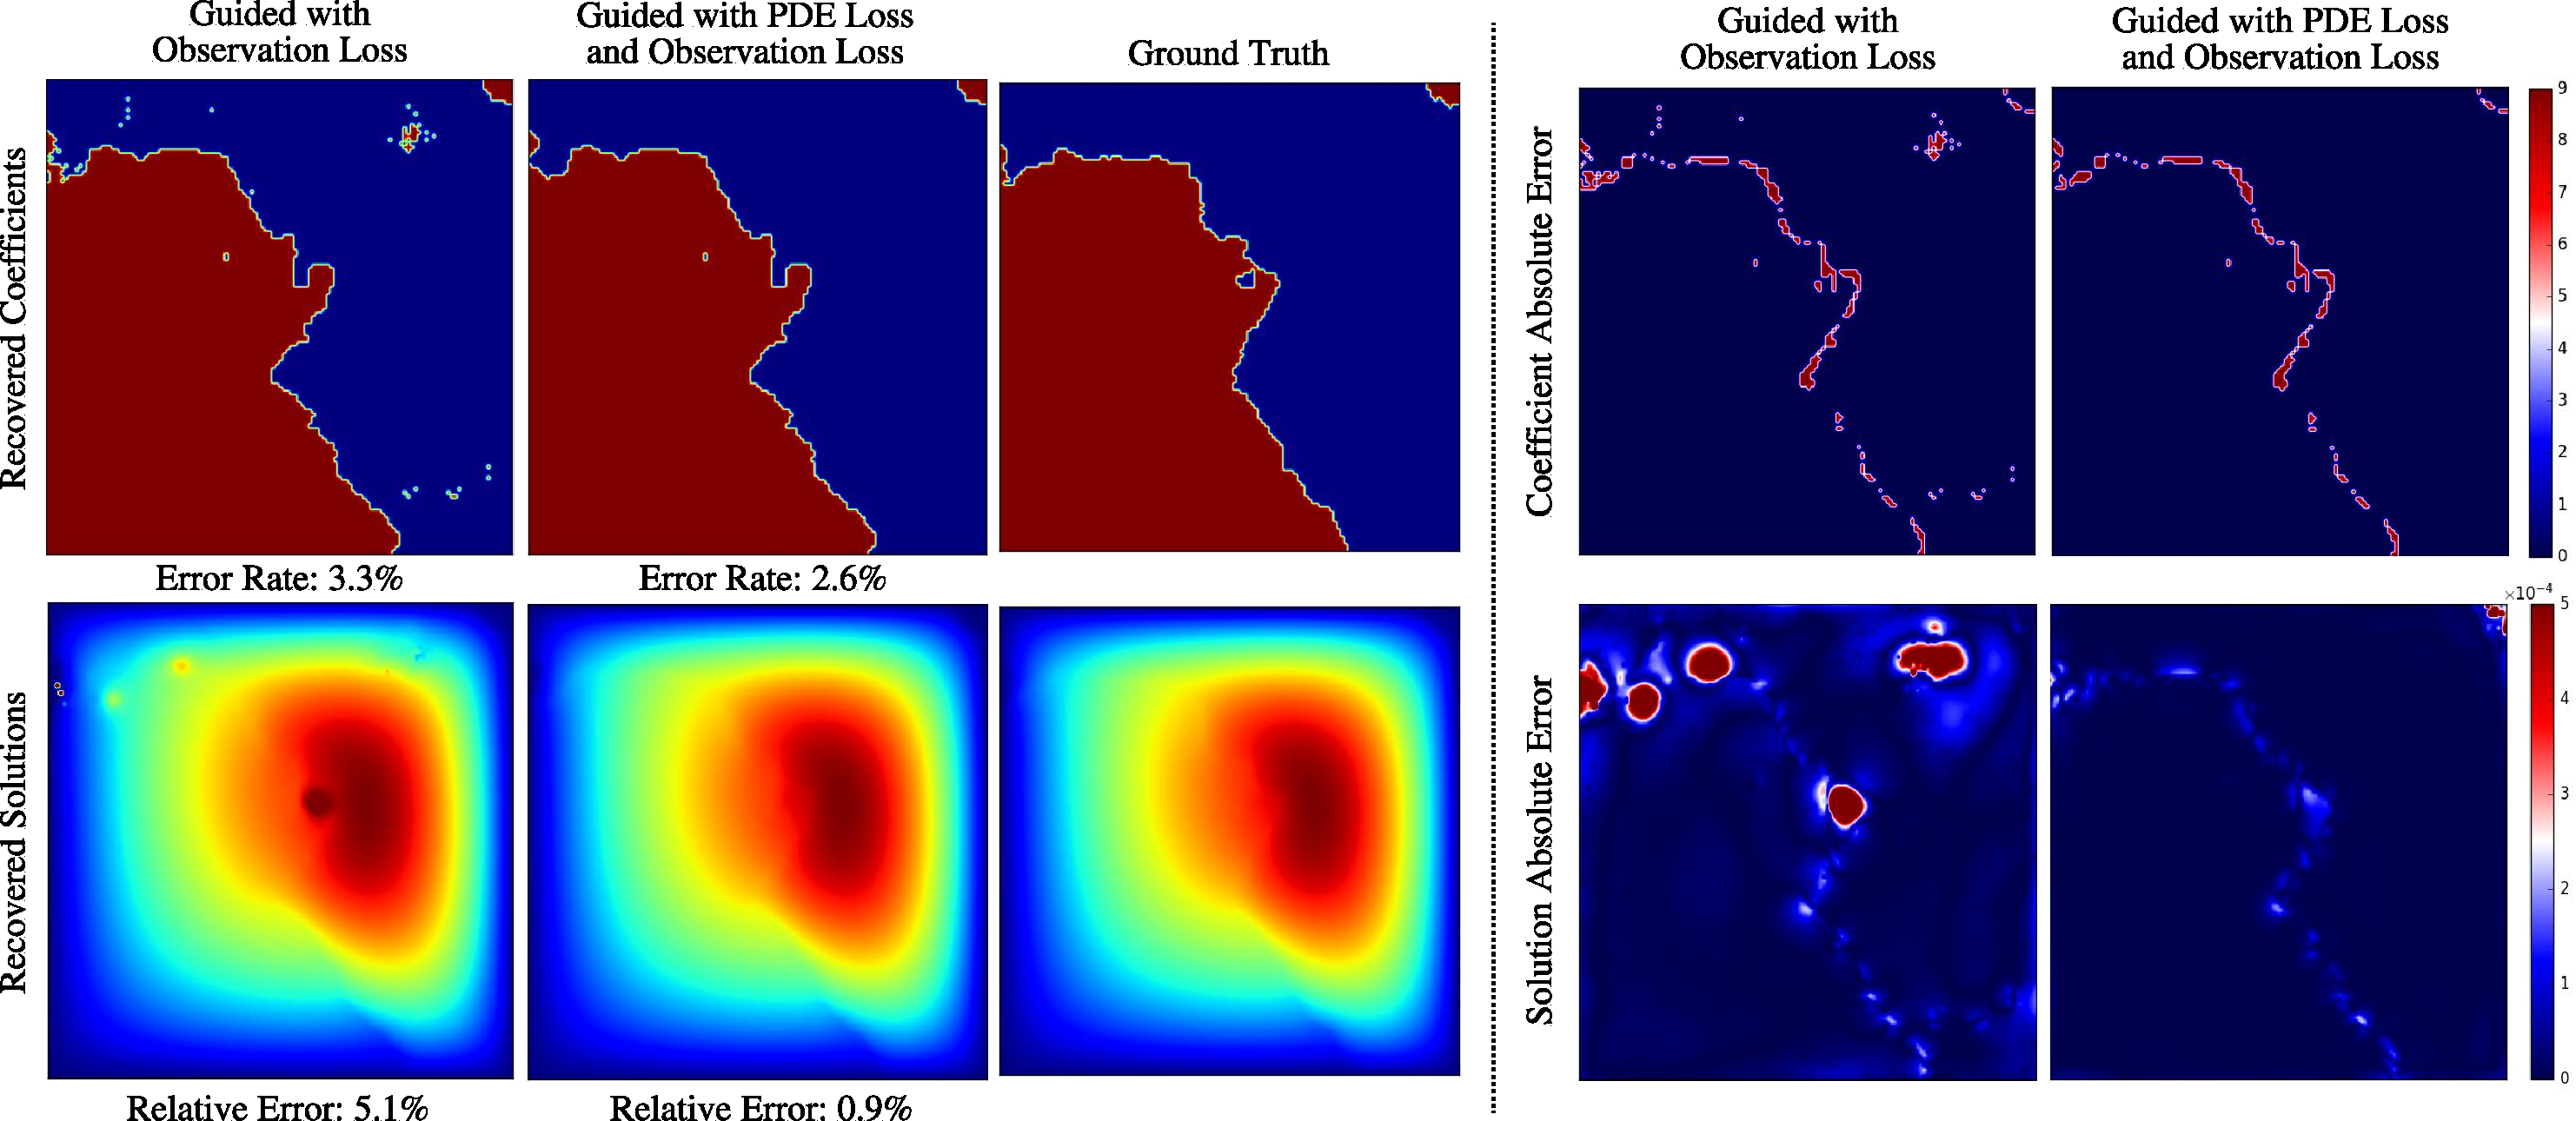
\includegraphics[width=0.99\textwidth]{figs/darcy/darcy_with_without_pde.pdf}
        \subcaption{Recovered coefficients, solutions, and corresponding absolute errors of Darcy Flow.}
    \end{subfigure}
\end{figure}



\begin{figure}[H]\ContinuedFloat
    \centering
    \begin{subfigure}{\textwidth}
        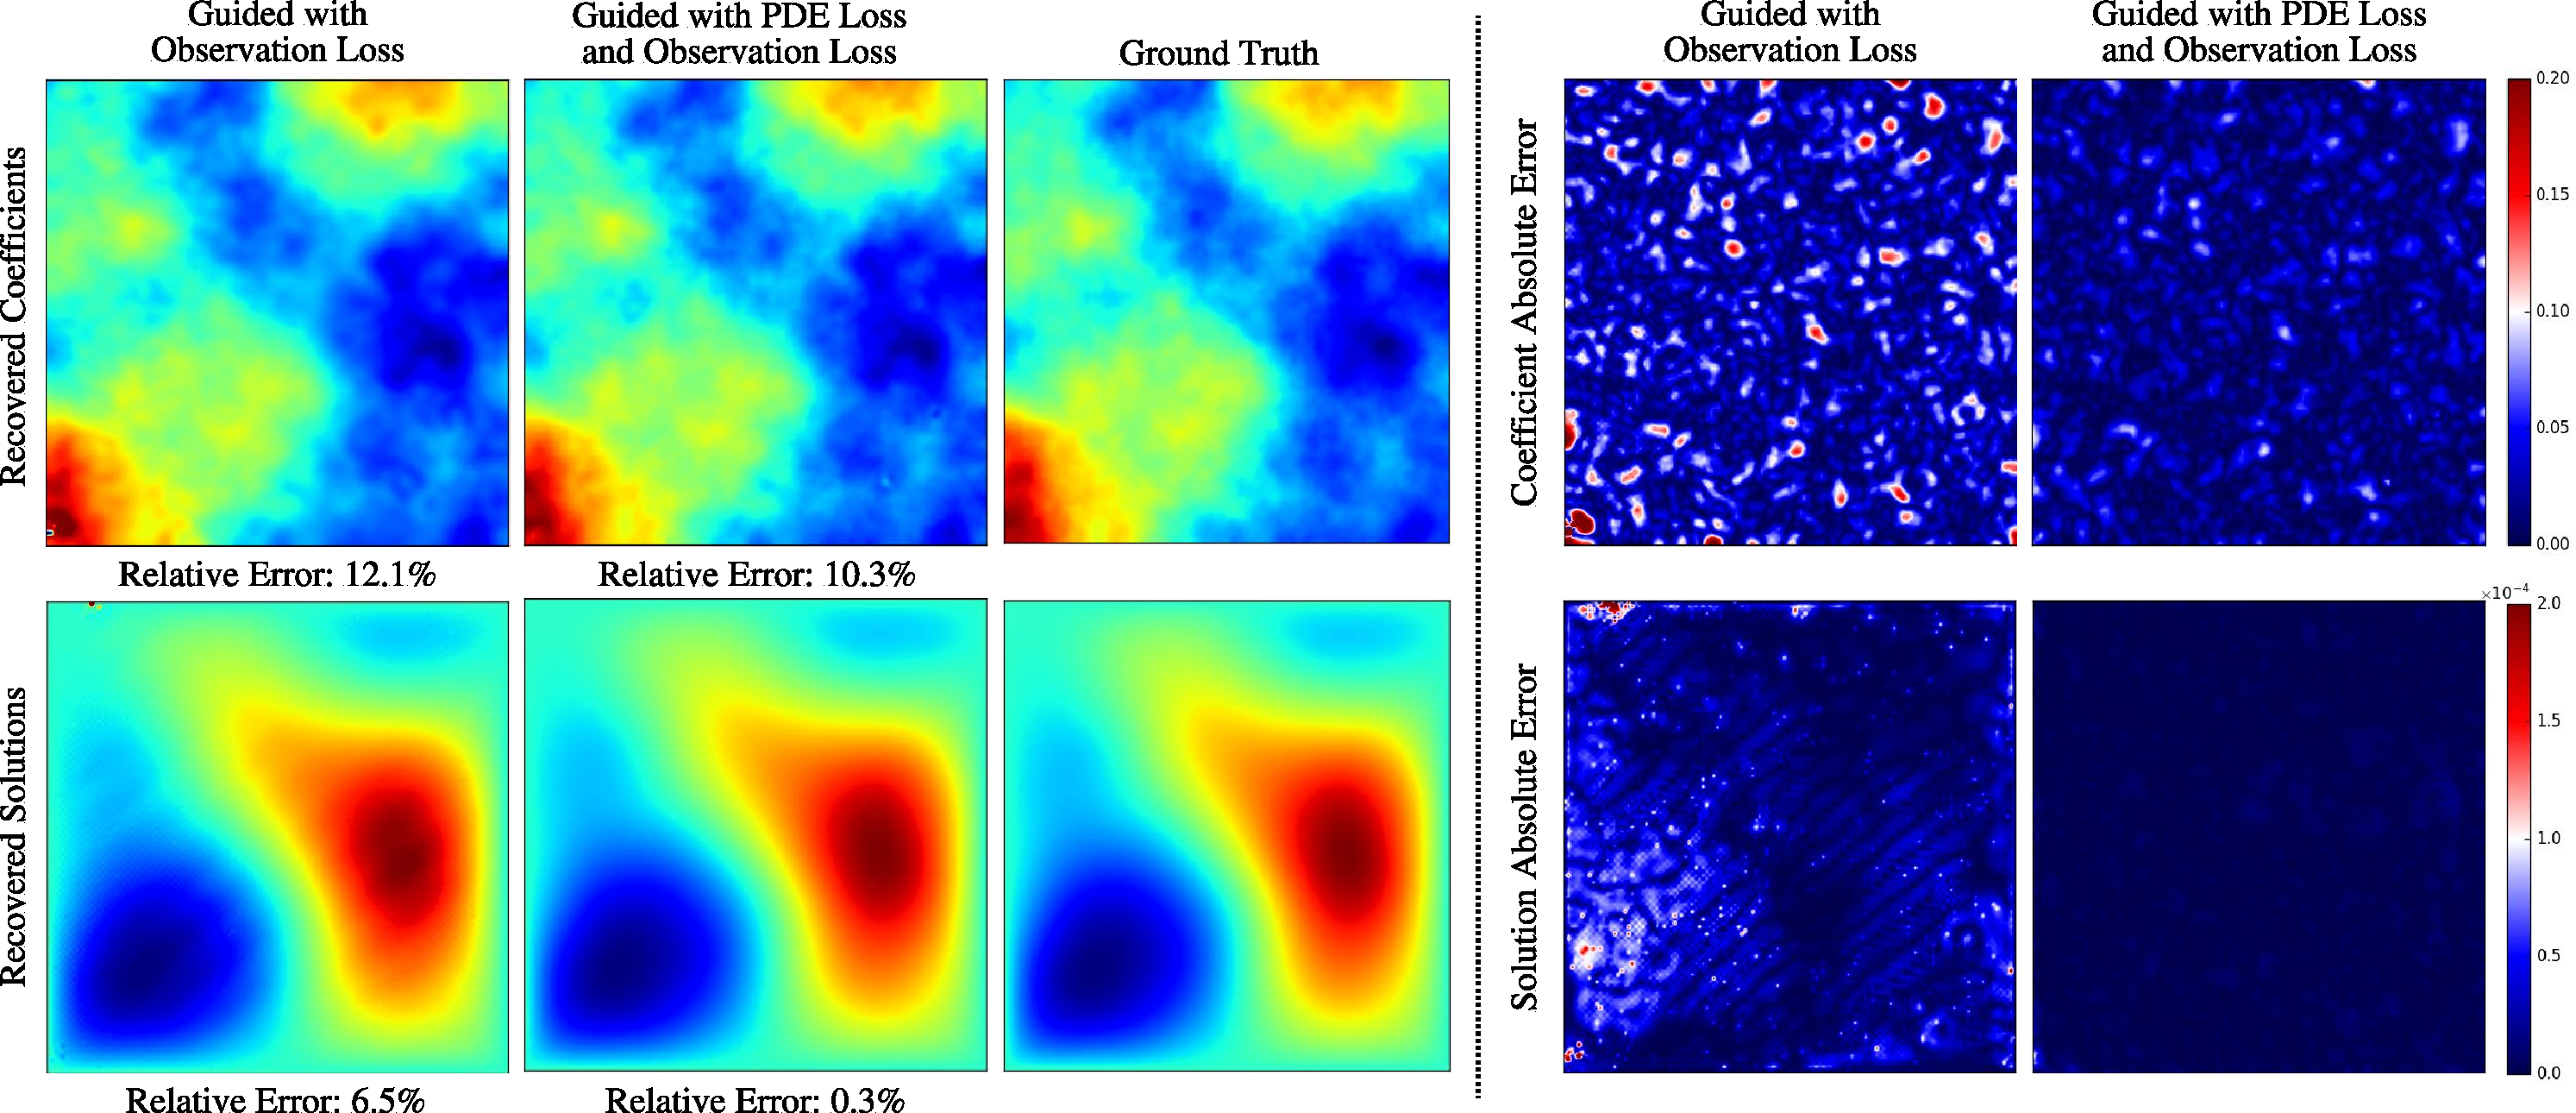
\includegraphics[width=0.99\textwidth]{figs/poisson/poisson_with_without_pde.pdf}
        \subcaption{Recovered coefficients, solutions, and corresponding absolute errors of Poisson equation.}
        \vspace{0.8em}
        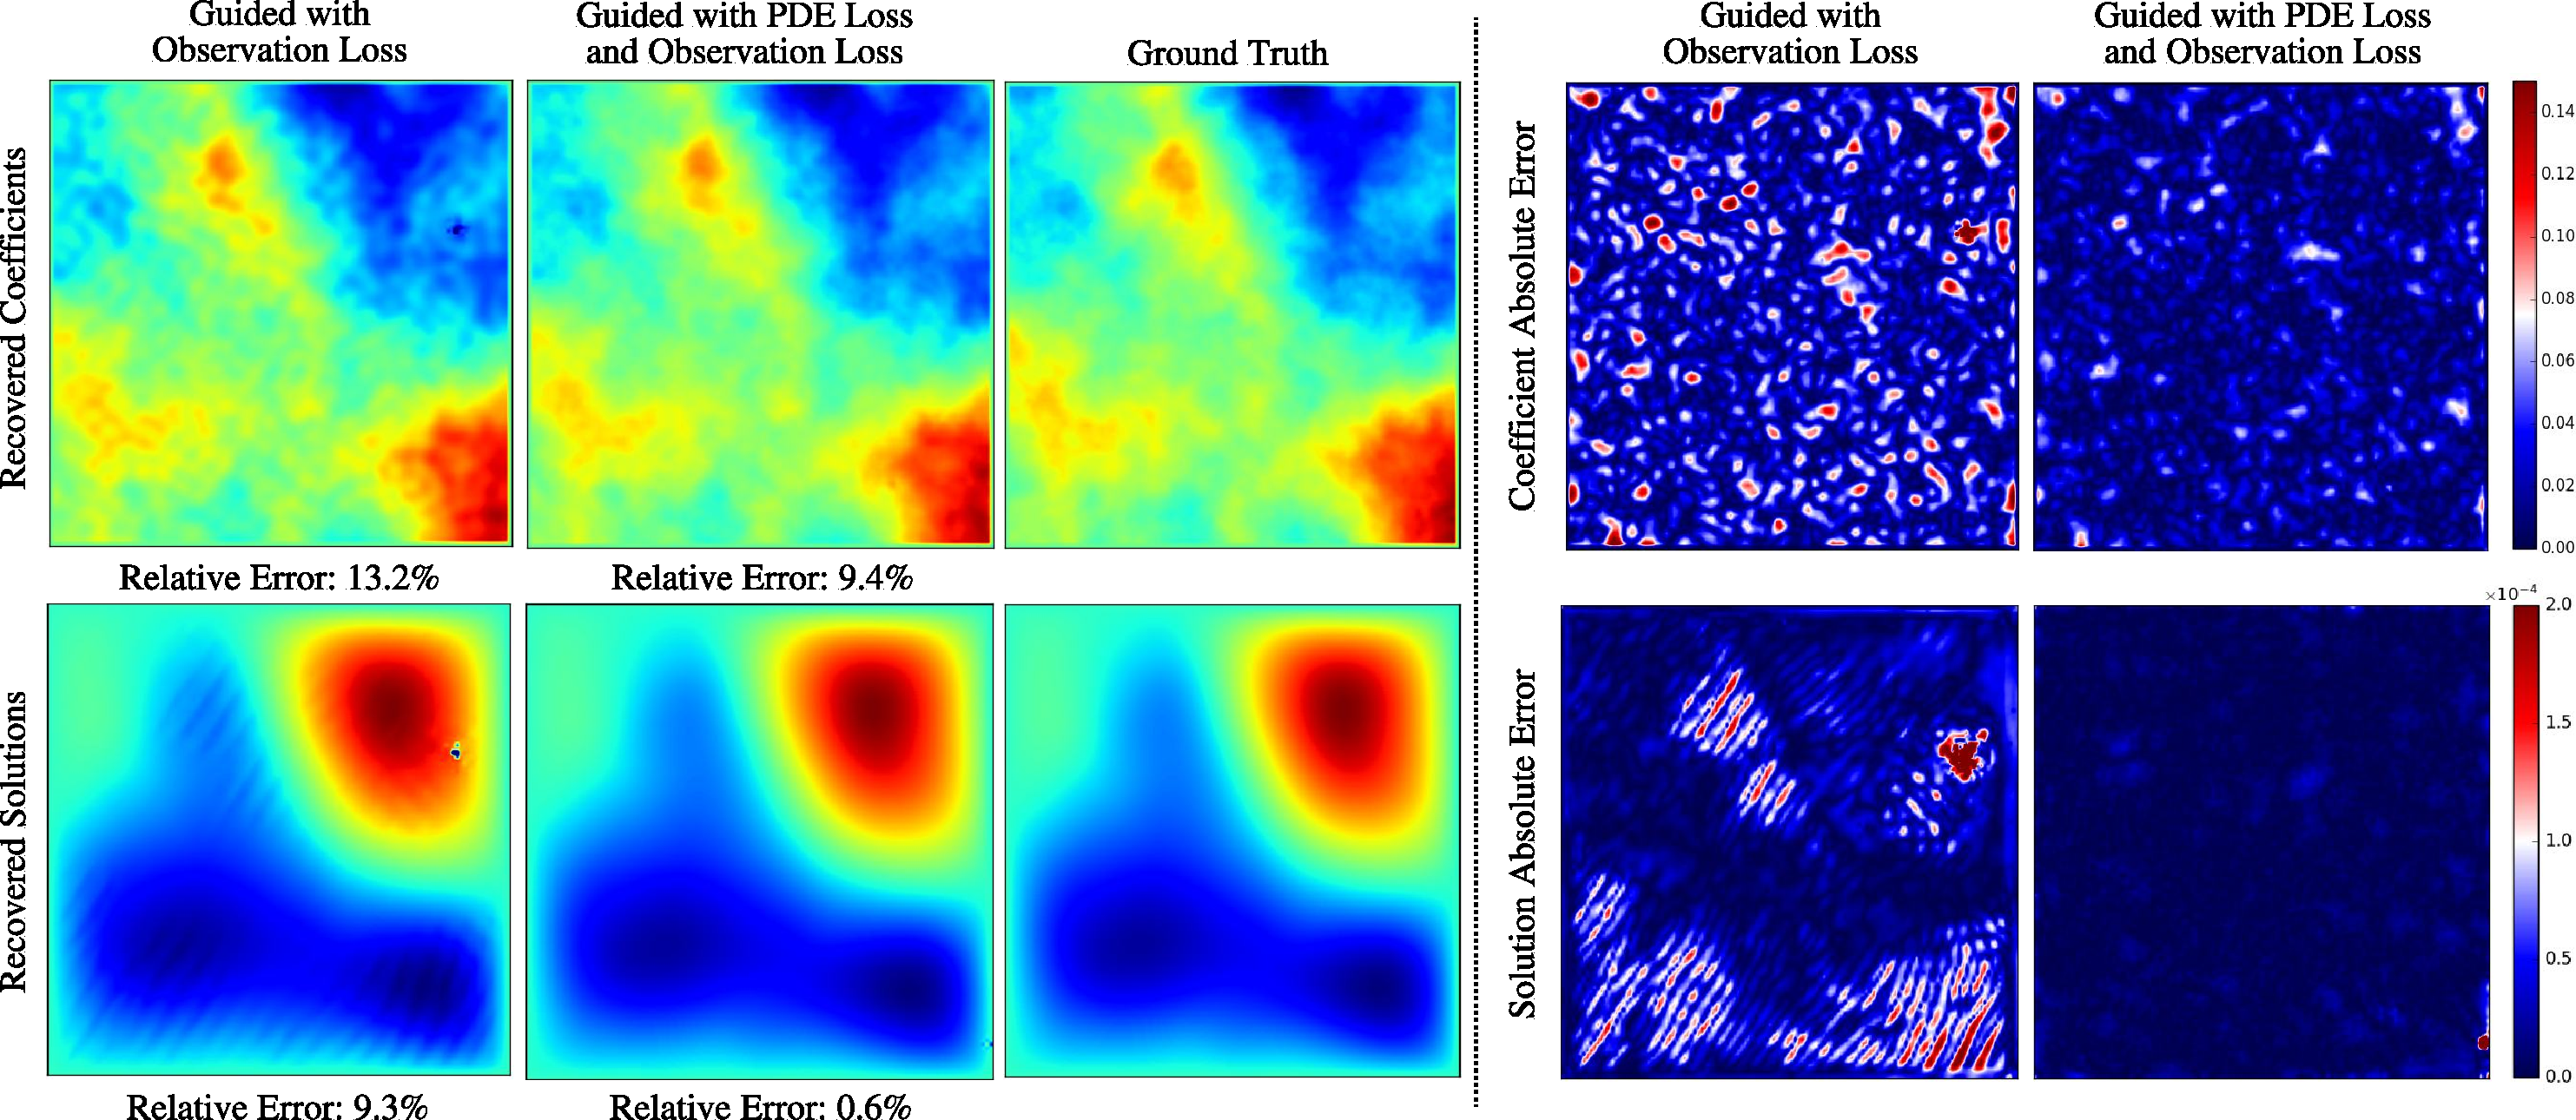
\includegraphics[width=0.99\textwidth]{figs/helmholtz/helmholtz_with_without_pde.pdf}
        \subcaption{Recovered coefficients, solutions, and corresponding absolute errors of Helmholtz equation.}
    \end{subfigure}
    \caption{Recovered coefficients, solutions, and their corresponding visualized absolute errors for various PDE families.}
    \label{fig:static_all_guidance}
\end{figure}



\vspace{-0.5em}
\section{Additional Results on All PDEs with Sparse Observation}\label{sec:all-sparse}
\vspace{-0.3em}

We present the recovered results of another Burgers' equation in Fig. \ref{fig:burger-2}. DiffusionPDE outperforms all other methods with 5 sensors for continuous observation. We also present the recovered results for both the forward and inverse problems of all other PDEs with sparse observations, as shown in Fig. \ref{fig:all-pdes}. Specifically, we solve the forward and inverse problems for the Darcy Flow, Poisson equation, Helmholtz equation, and non-bounded Navier-Stokes equation using 500 random points observed in either the solution space or the coefficient space. Additionally, for the bounded Navier-Stokes equation, we observe 1\% of the points in the velocity field. Our findings indicate that DiffusionPDE outperforms all other methods, providing the most accurate solutions.

\paragraph{Additional Data Setting for Darcy Flow}

To further demonstrate the generalization capability of our model, we conducted additional tests on different data settings for Darcy Flow. In Fig. \ref{fig:darcy-20and26}, we solve the forward and inverse problems of Darcy Flow with 500 observation points, adjusting the binary values of $a$ to 20 and 16 instead of the original 12 and 3 in Section \ref{sec:data_generation}, i.e.,
\begin{equation*}
    \left\{
    \begin{aligned}
        a(x)&=20, \quad&&\text{if }\mu(x)\geq0\\
        a(x)&=16, &&\text{if }\mu(x)<0
    \end{aligned}
    \right.
\end{equation*}
Our results indicate that DiffusionPDE performs equally well under these varied data settings, showcasing its robustness and adaptability.

\begin{figure}[H]
    \centering
    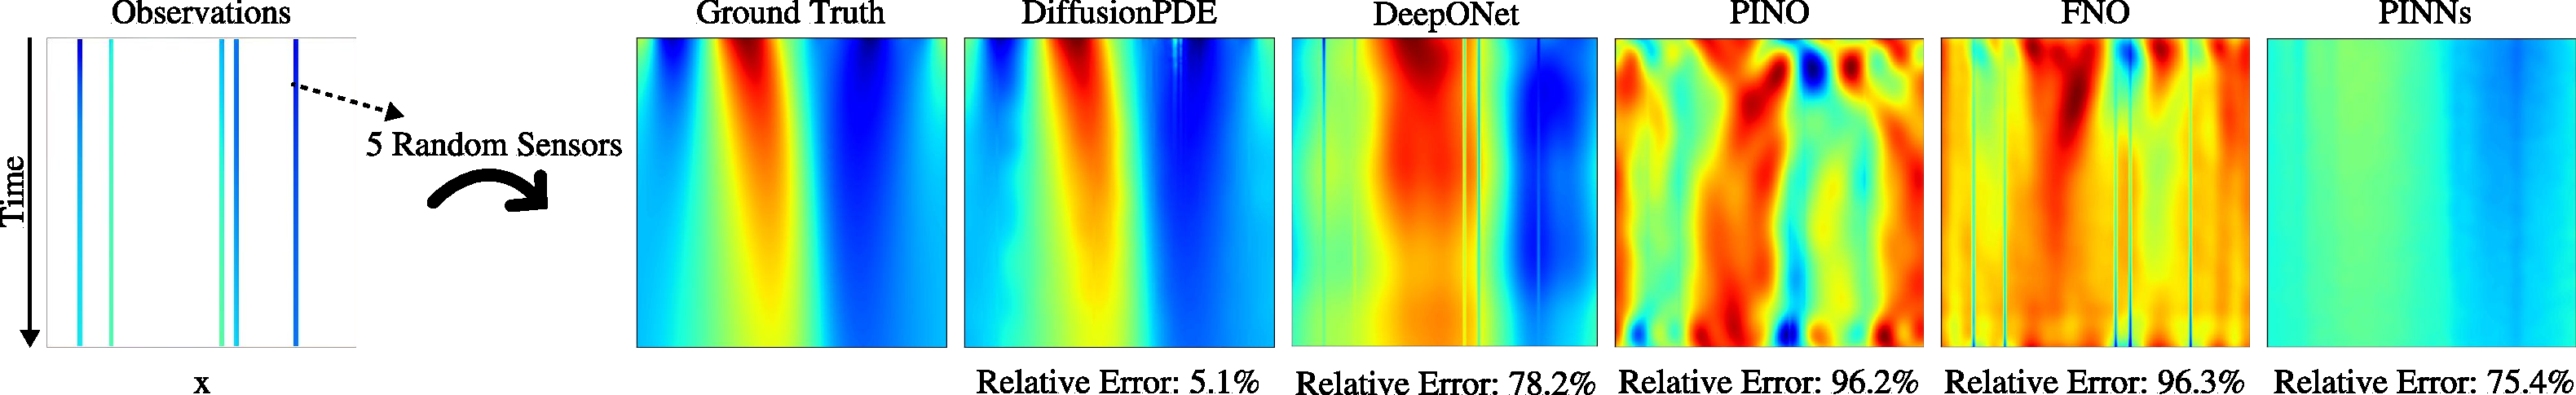
\includegraphics[width=0.99\textwidth]{figs/burger/burger_all_methods_2_updated.pdf}
    \caption{Results of another Burgers' equation recovered by 5 sensors throughout the time interval.}
    \label{fig:burger-2}
\end{figure}
\vspace{-1em}

\begin{figure}[H]
    \centering
        \begin{subfigure}{\textwidth}
        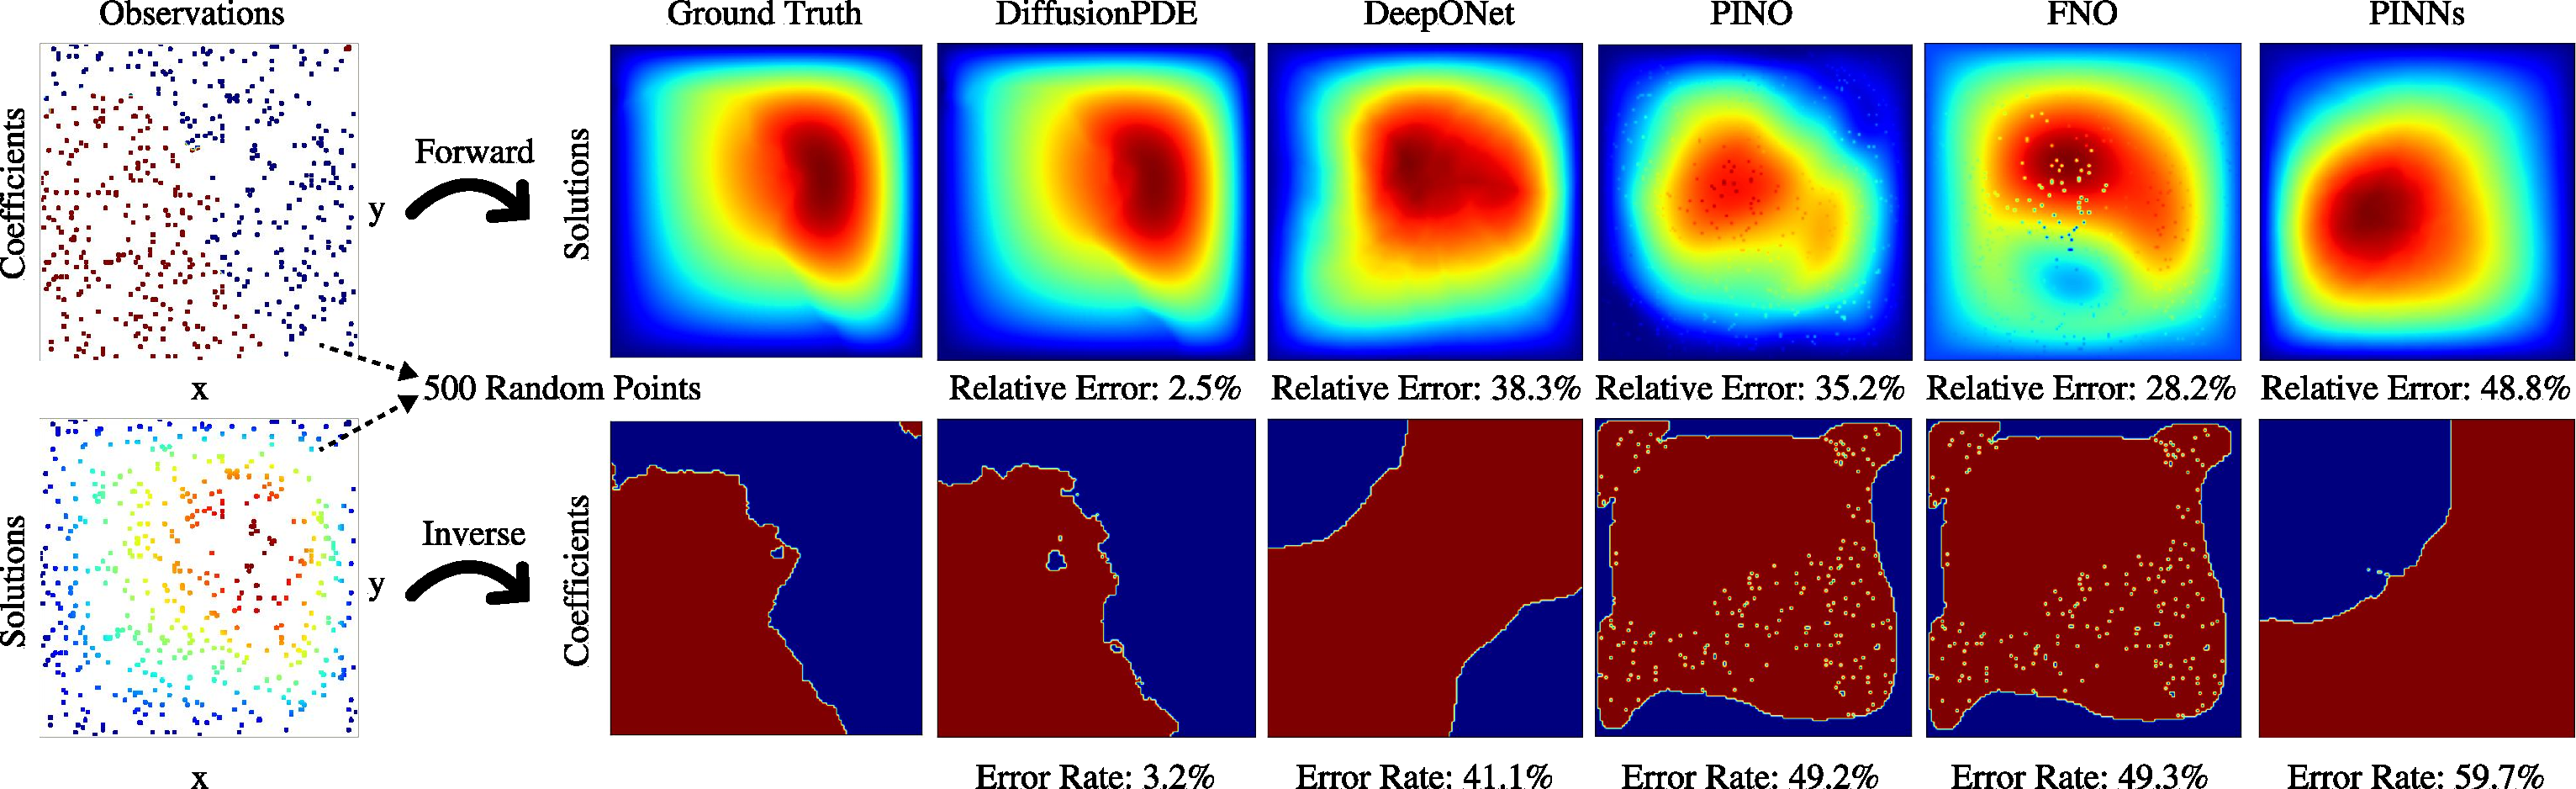
\includegraphics[width=0.99\textwidth]{figs/darcy/darcy_allmethods.pdf}
        \subcaption{Forward and inverse results of Darcy Flow recovered by 500 observation points.}
        \vspace{0.1em}
        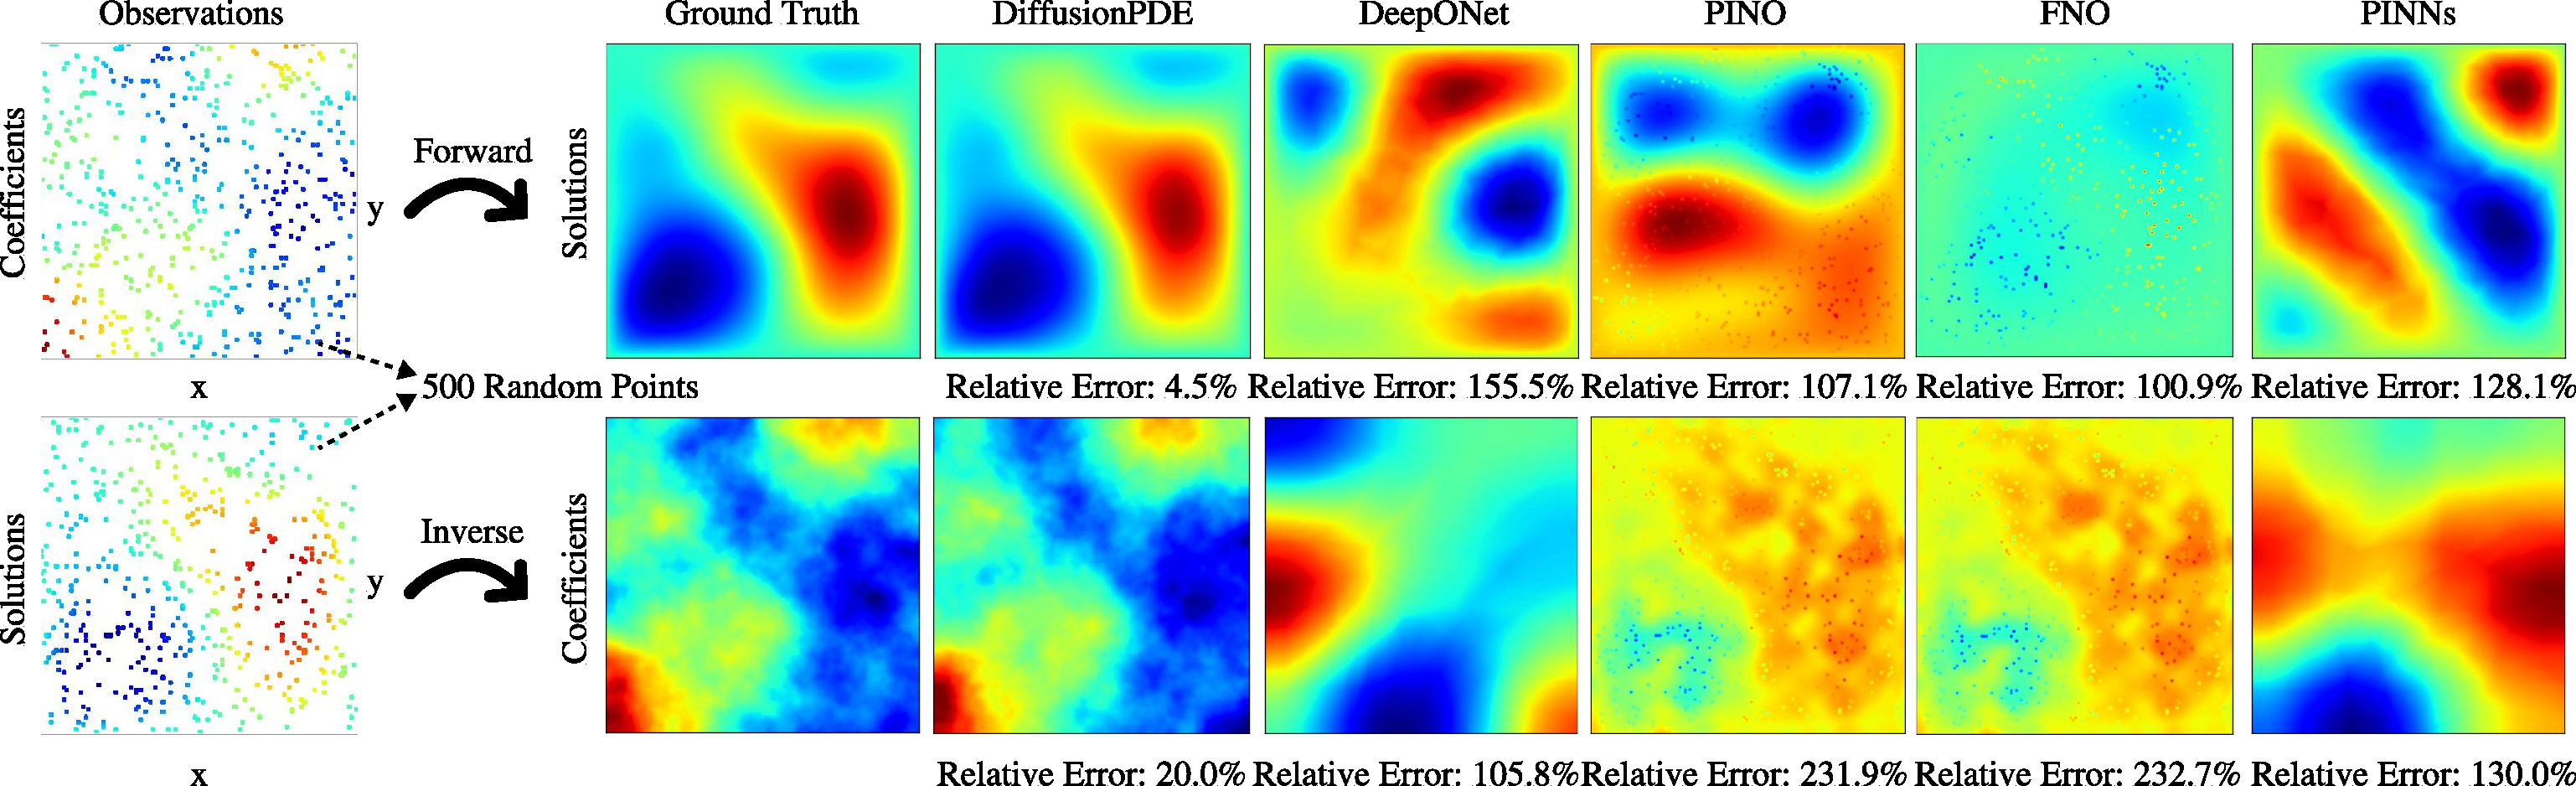
\includegraphics[width=0.99\textwidth]{figs/poisson/poisson_allmethods.pdf}
        \subcaption{Forward and inverse results of Poisson equation recovered by 500 observation points.}
        \vspace{0.1em}
        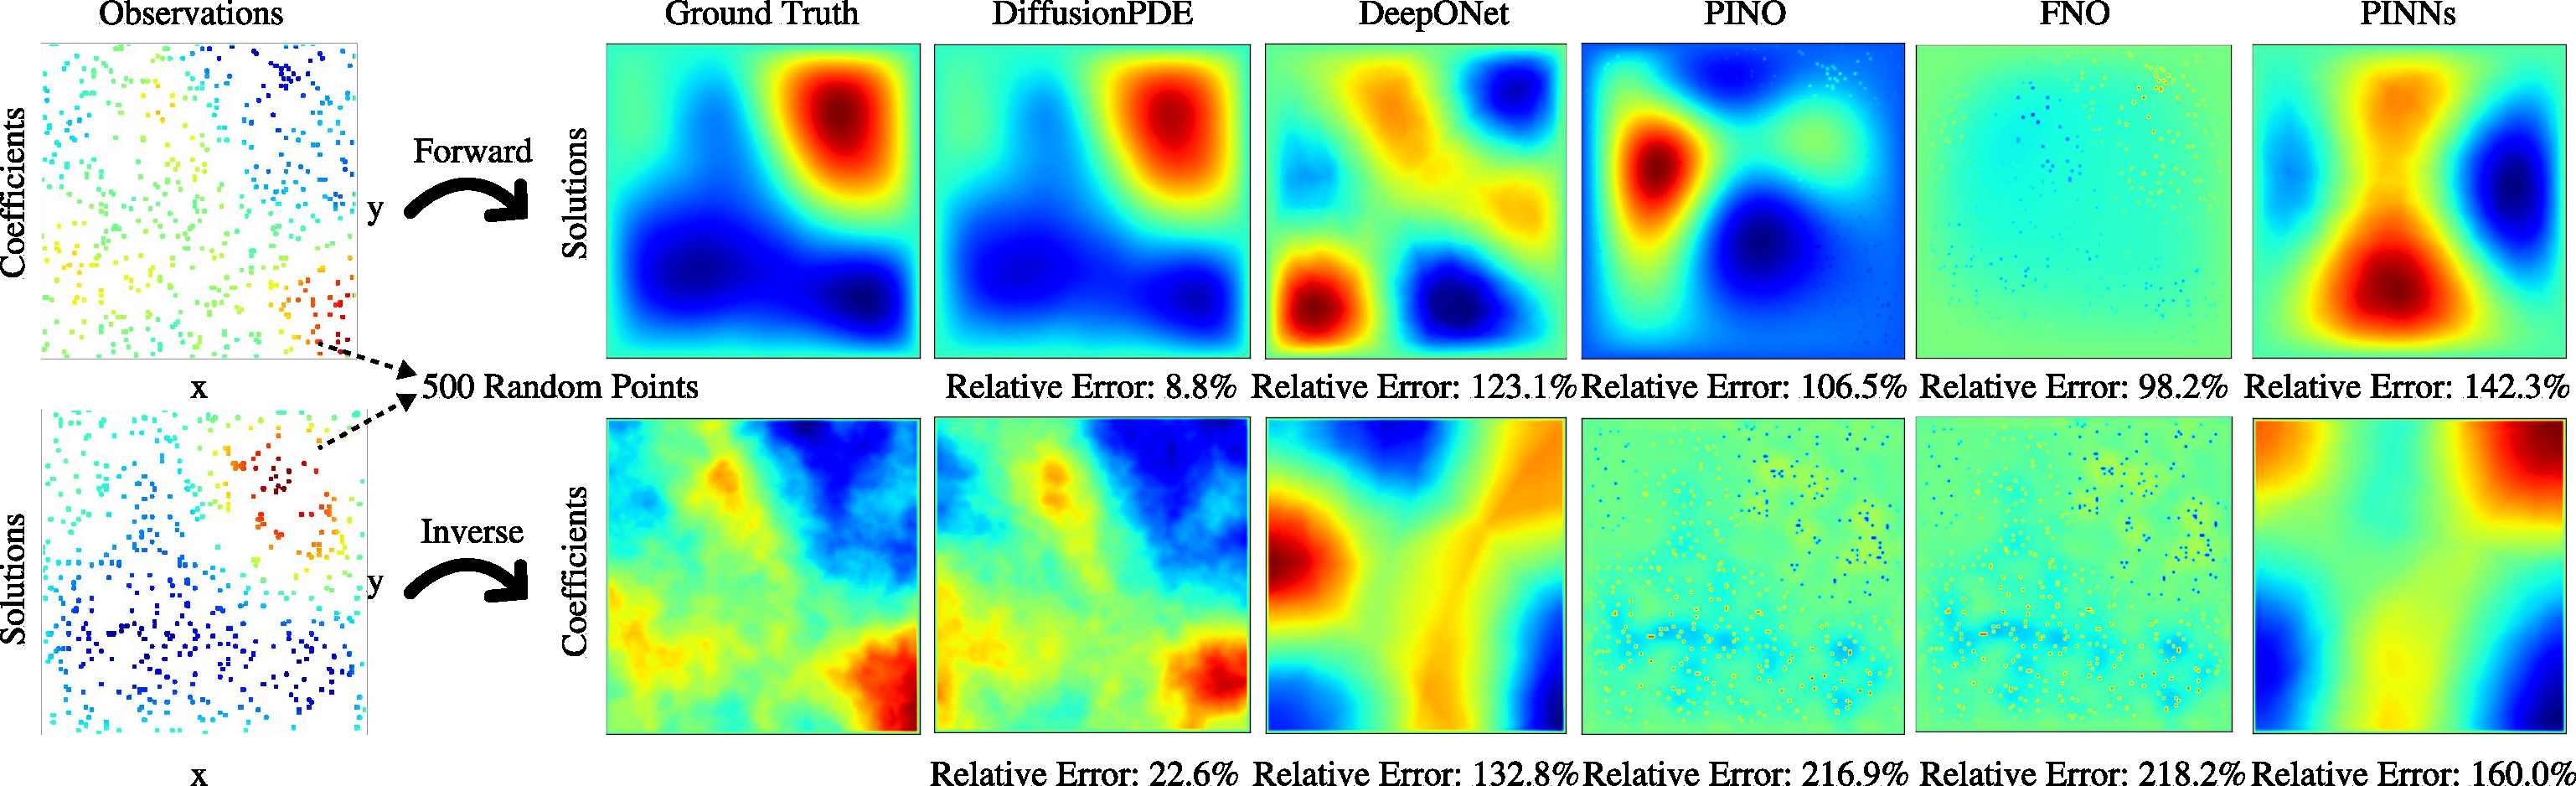
\includegraphics[width=0.99\textwidth]{figs/helmholtz/helmholtz_allmethods.pdf}
            \subcaption{Forward and inverse results of Helmholtz equation recovered by 500 observation points.}
            \vspace{0.1em}
            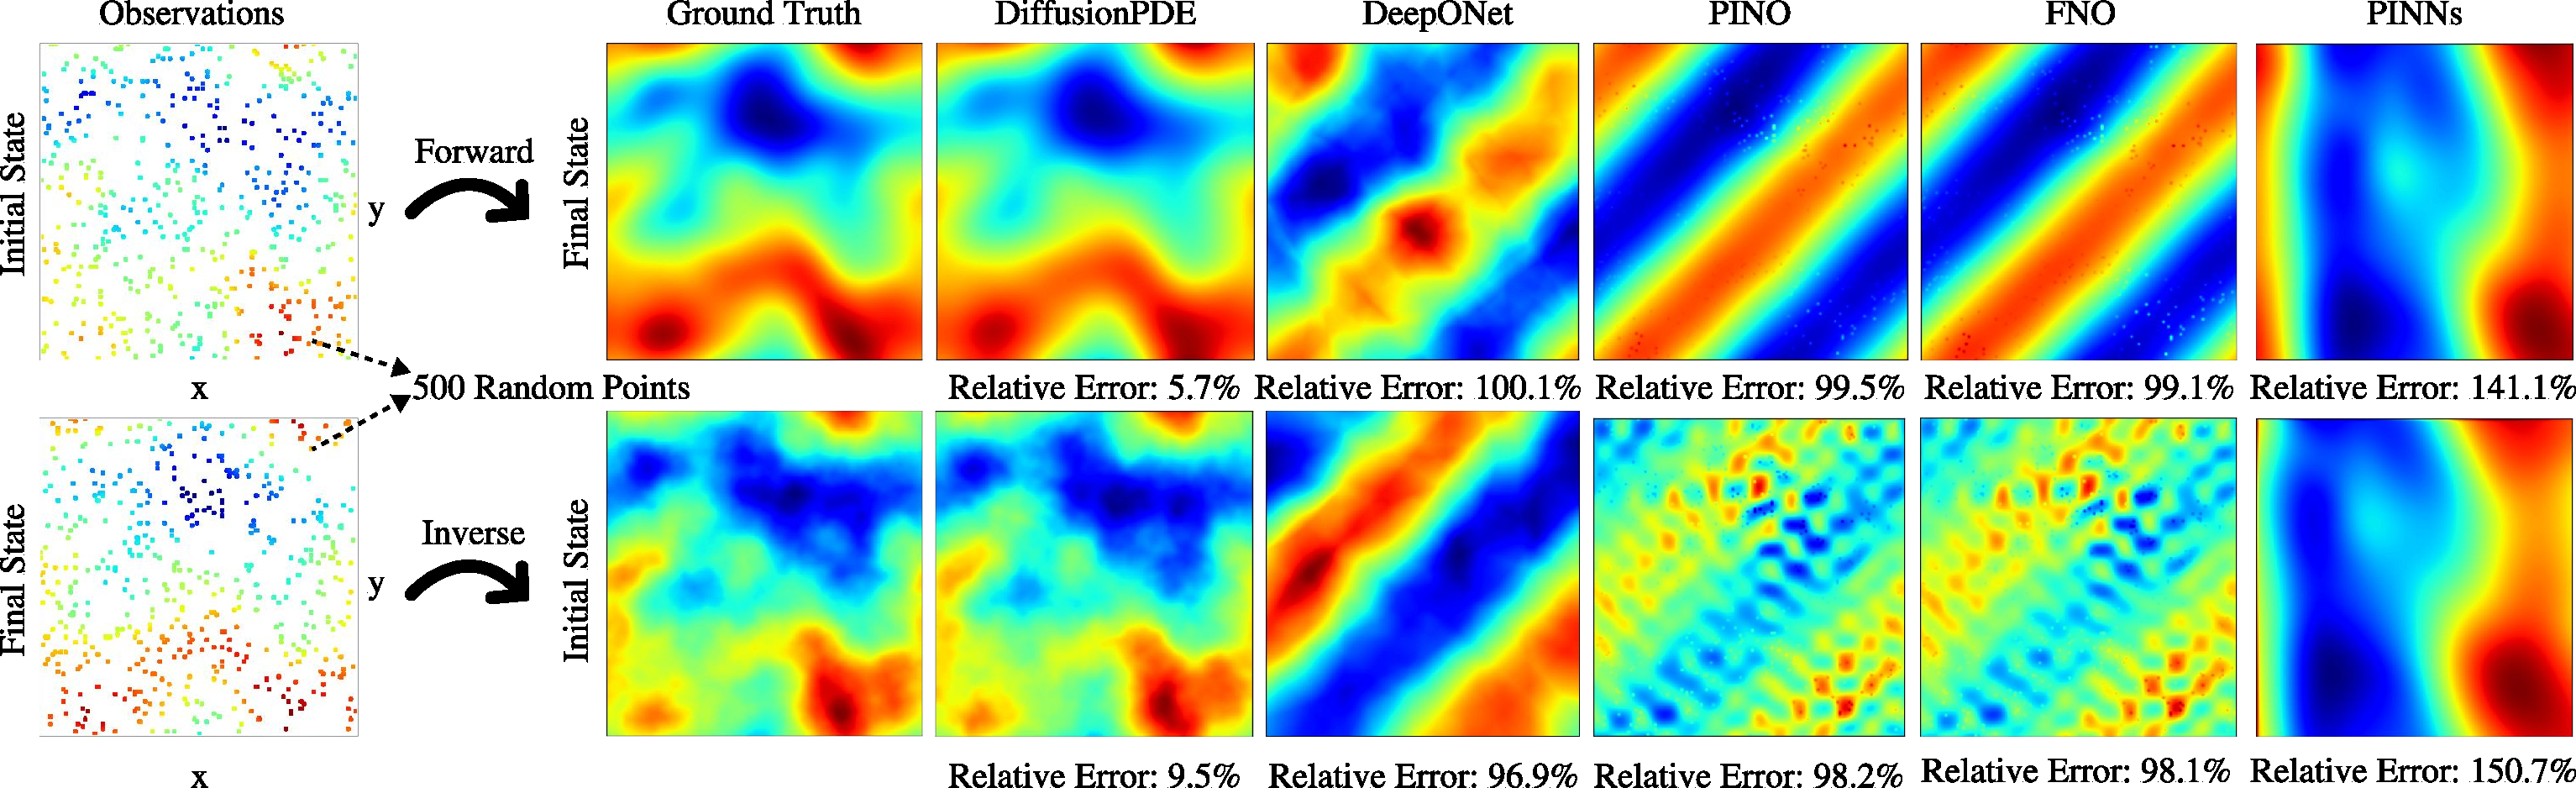
\includegraphics[width=0.99\textwidth]{figs/ns/non-bounded_ns_allmethods_2.pdf}
            \subcaption{Forward and inverse results of another non-bounded Navier-Stokes equation recovered by 500 observation points.}
            
        \end{subfigure}
    
\end{figure}

\begin{figure}[H]\ContinuedFloat
    \centering
    \begin{subfigure}{\textwidth}
    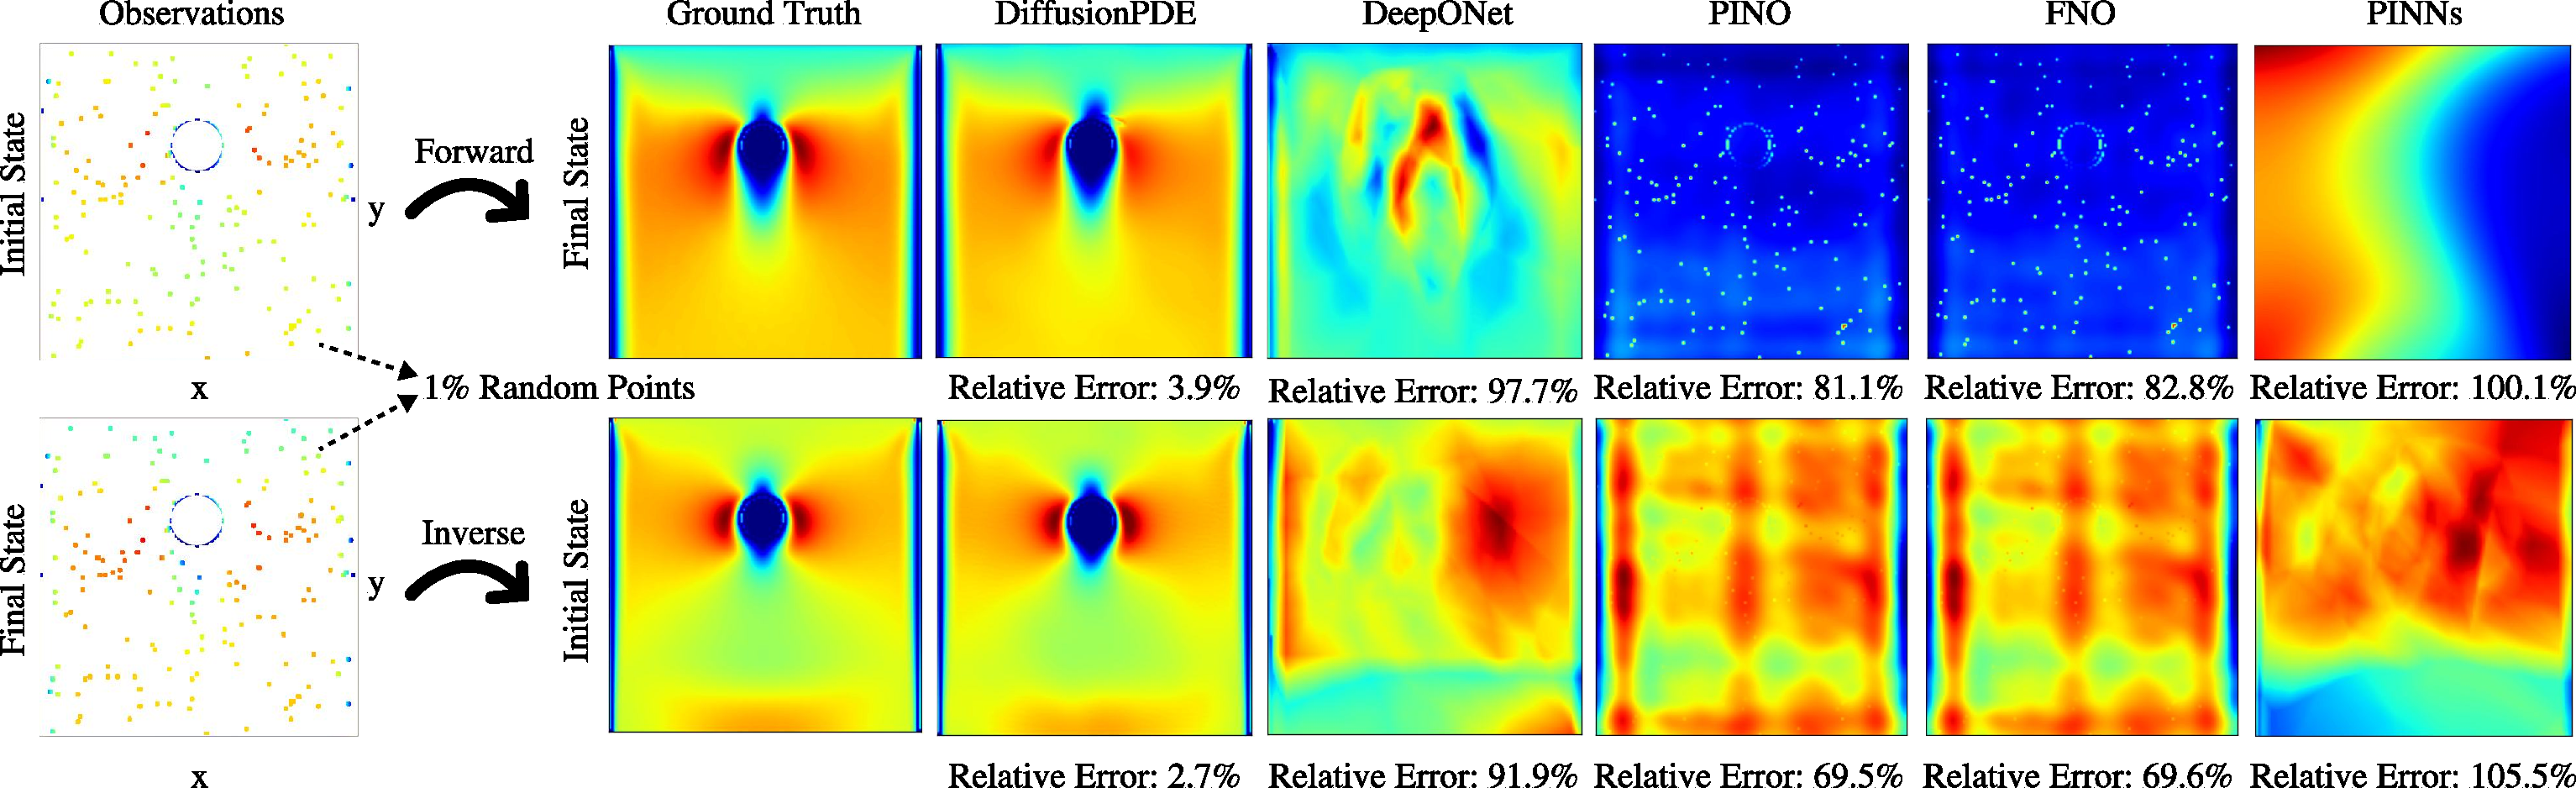
\includegraphics[width=0.99\textwidth]{figs/ns/bounded_ns_allmethods.pdf}
            \subcaption{Forward and inverse results of bounded Navier-Stokes equation recovered by 1\% observation points.}
            \vspace{0.8em}
        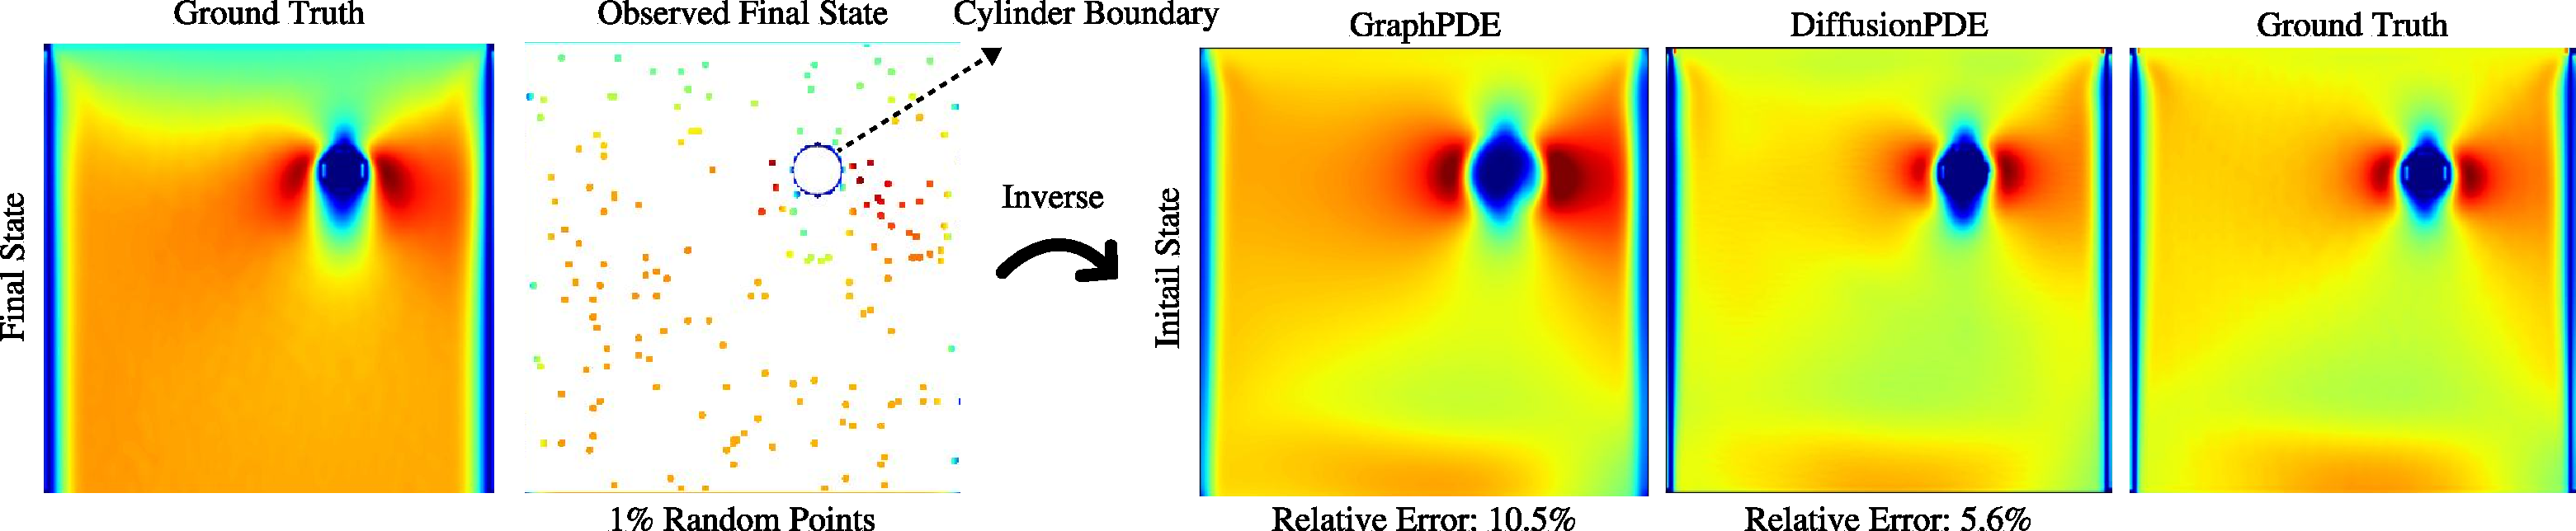
\includegraphics[width=0.99\textwidth]{figs/ns/bounded_NS_withGraphPDE_2.pdf}
            \subcaption{Inverse results of DiffusionPDE and GraphPDE of another bounded Navier-Stokes equation recovered by 1\% observation points and the known boundary of the cylinder.}
        
    \end{subfigure}
    \caption{Results of forward and inverse problems for different PDE families with sparse observation.}
    \label{fig:all-pdes}
    \vspace{-0.5em}
\end{figure}


\begin{figure}[H]
    \centering
    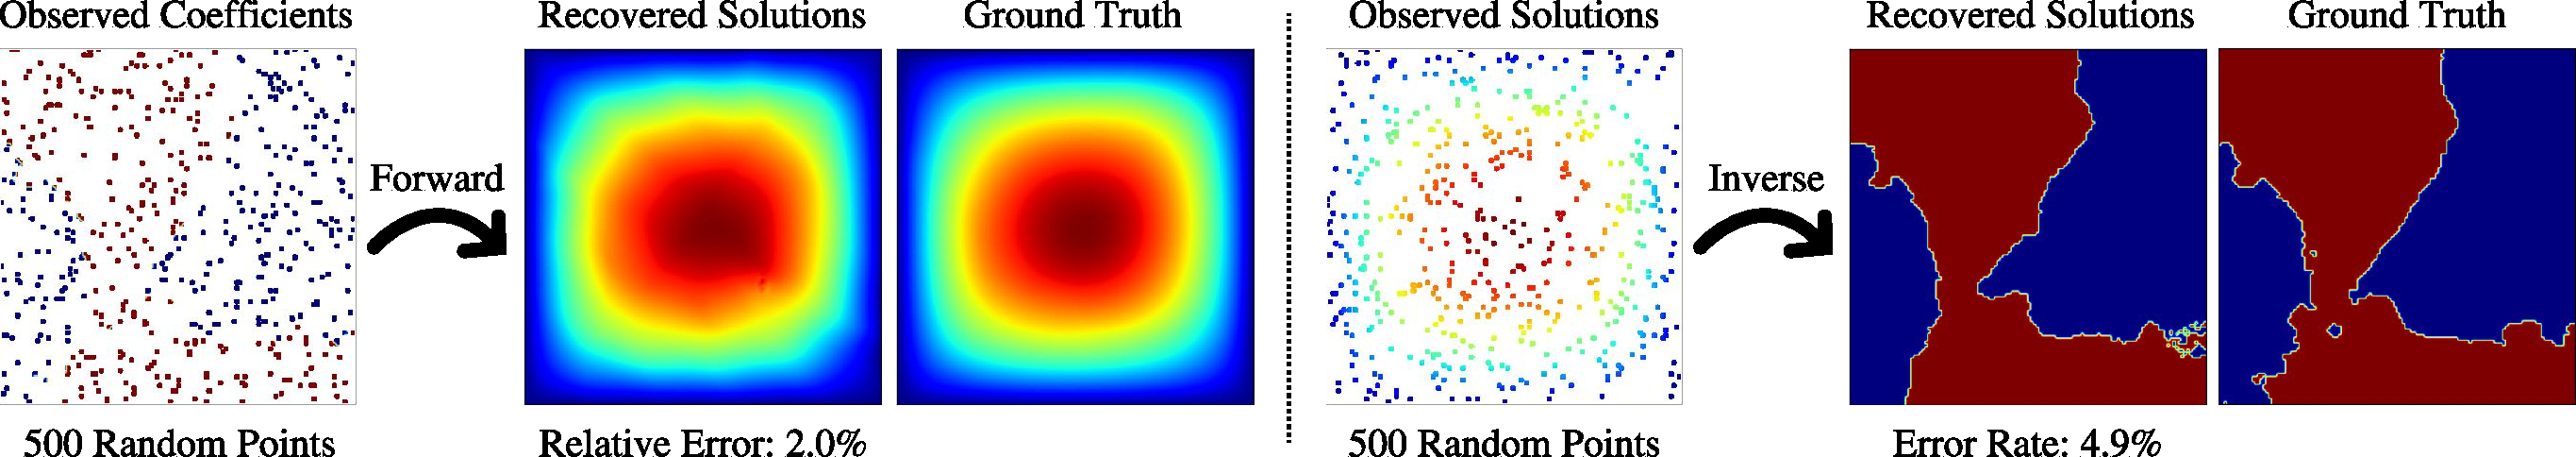
\includegraphics[width=0.99\textwidth]{figs/darcy/darcy_20and16.pdf}
    \caption{Forward and inverse results of Darcy Flow recovered by 500 observation points under a different data setting.}
    \label{fig:darcy-20and26}
    \vspace{-1.0em}
\end{figure}
\begin{figure}[H]
    \centering
    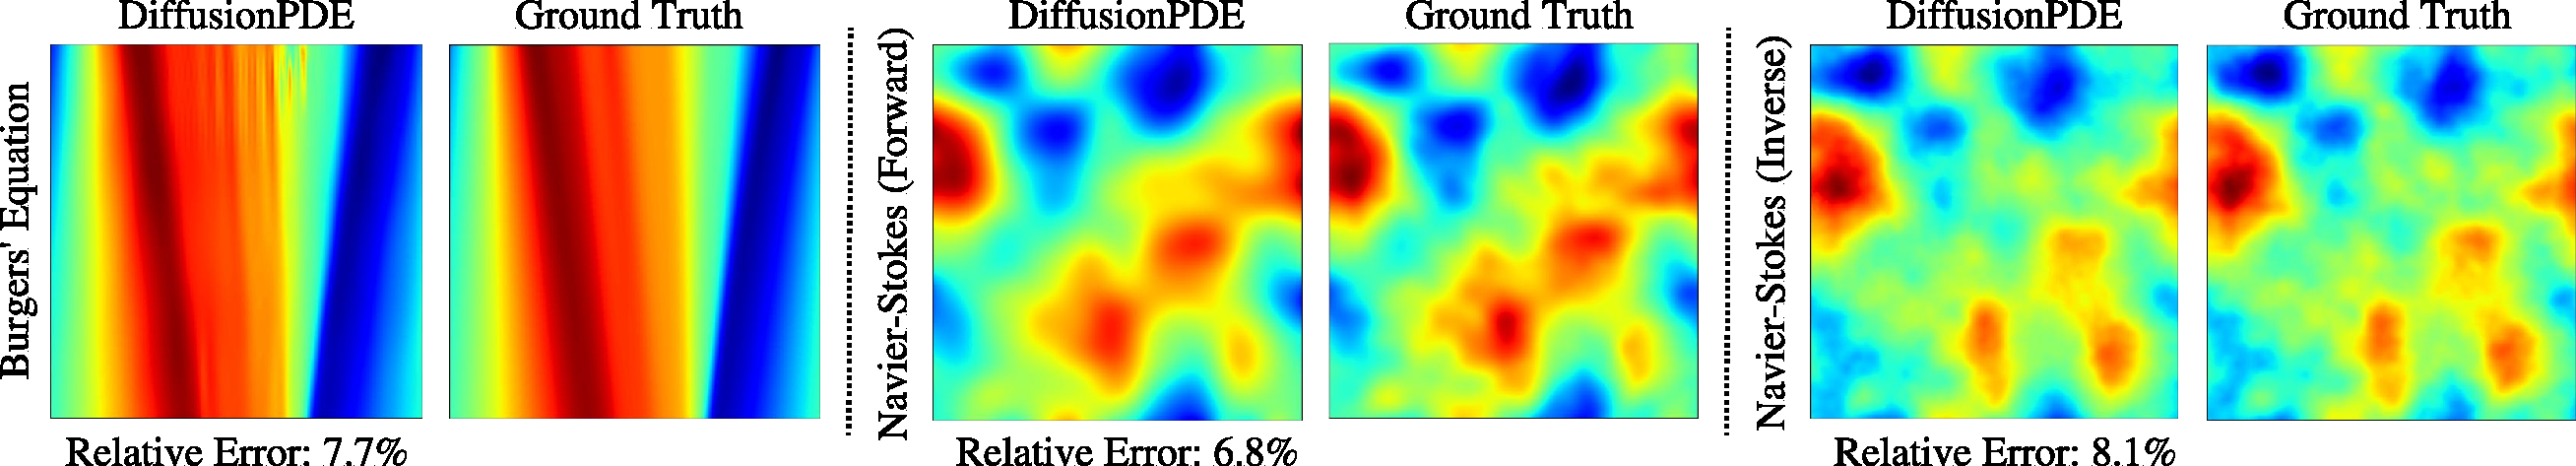
\includegraphics[width=0.99\textwidth]{figs/rebuttal/DiffusionPDE_21.pdf}
    \caption{Results of Navier-Stokes equation and Burgers' equation with 10 times smaller viscosity.}
    \label{fig:10-times-smaller-visc}
    \vspace{-0.5em}
\end{figure}

\vspace{-1.0em}
\paragraph{Additional Data Setting for Non-bounded Navier-Stokes Equation and Burgers’ Equation}

We also test DiffusionPDE on the Burgers’ equation with a viscosity of $1\times 10^{-3}$ and on the non-bounded Navier-Stokes equation with a viscosity of $1\times 10^{-4}$, which are 10 times smaller than the ones in the main paper, as shown in Fig. \ref{fig:10-times-smaller-visc}. For the Burgers’ equation, we are able to recover the full time interval with 5 fixed sensors at a relative error of approximately $6\%$, which is close to the error of approximately $2\sim 5\%$ in the main paper. For the Navier-Stokes equation, we can solve the forward and inverse problems with relative errors of approximately $7\%$ and $9\%$, respectively, using 500 observation points. The errors are also close to the ones in the main paper, where the forward and inverse errors of Navier-Stokes equation are approximately $7\%$ and $10\%$.


\vspace{-0.3em}
\section{Solving Forward and Inverse Problems with Full Observation}\label{sec:all-full}
\vspace{-0.2em}

We have also included the errors of all methods when solving both the forward and inverse problems with full observation, as displayed in Table \ref{table:merged_results_full}.

\begin{table}[H]
    \vspace{-1em}
    \caption{Relative errors of solutions (or final states) and coefficients (or initial states) when solving forward and inverse problems with full observations. Error rates are used for the inverse problem of Darcy Flow.}
    \label{table:merged_results_full}
    \centering
    \begin{tabular}{p{2cm}llccccc}
        \toprule
        & & DiffusionPDE & PINO & DeepONet & PINNs & FNO \\
        \midrule
        \multirow{2}{2cm}{Darcy Flow} & Forward & \textbf{2.2\%} & 4.0\% & 12.3\% & 15.4\% & 5.3\% \\
        & Inverse & \textbf{2.0\%} & 2.1\% & 8.4\% & 10.1\% & 5.6\% \\
        \midrule
        \multirow{2}{2cm}{Poisson} & Forward & \textbf{2.7\%} & 3.7\% & 14.3\% & 16.1\% & 8.2\% \\
        & Inverse & \textbf{9.8\%} & 10.2\% & 29.0\% & 28.5\% & 13.6\% \\
        \midrule
        \multirow{2}{2cm}{Helmholtz} & Forward & \textbf{2.3\%} & 4.9\% & 17.8\% & 18.1\% & 11.1\% \\
        & Inverse & \textbf{4.0\%} & 4.9\% & 28.1\% & 29.2\% & 5.0\% \\
        \midrule
        \multirow{2}{2cm}{Non-bounded Navier-Stokes} & Forward & 6.1\% & \textbf{1.1\%} & 25.6\% & 27.3\% & 2.3\% \\
        & Inverse & 8.6\% & \textbf{6.8\%} & 19.6\% & 27.8\% & 6.8\% \\
        \midrule
        \multirow{2}{2cm}{Bounded Navier-Stokes} & Forward & \textbf{1.7\%} & 1.9\% & 13.3\% & 18.6\% & 2.0\% \\
        & Inverse & \textbf{1.4\%} & 2.9\% & 6.1\% & 7.6\% & 3.0\% \\
        \bottomrule
    \end{tabular}
\end{table}



 In general, DiffusionPDE and PINO outperform all other methods, and DiffusionPDE performs the best for all static PDEs. DiffusionPDE is capable of solving both forward and inverse problems with errors of less than 10\% for all classes of discussed PDEs and is comparable to the state-of-the-art. Results of all methods regarding Darcy Flow and non-bounded Navier-Stokes equation are included in Fig. \ref{fig:pdes-full}.

 \begin{figure}[H]
    \centering
    \begin{subfigure}{\textwidth}
    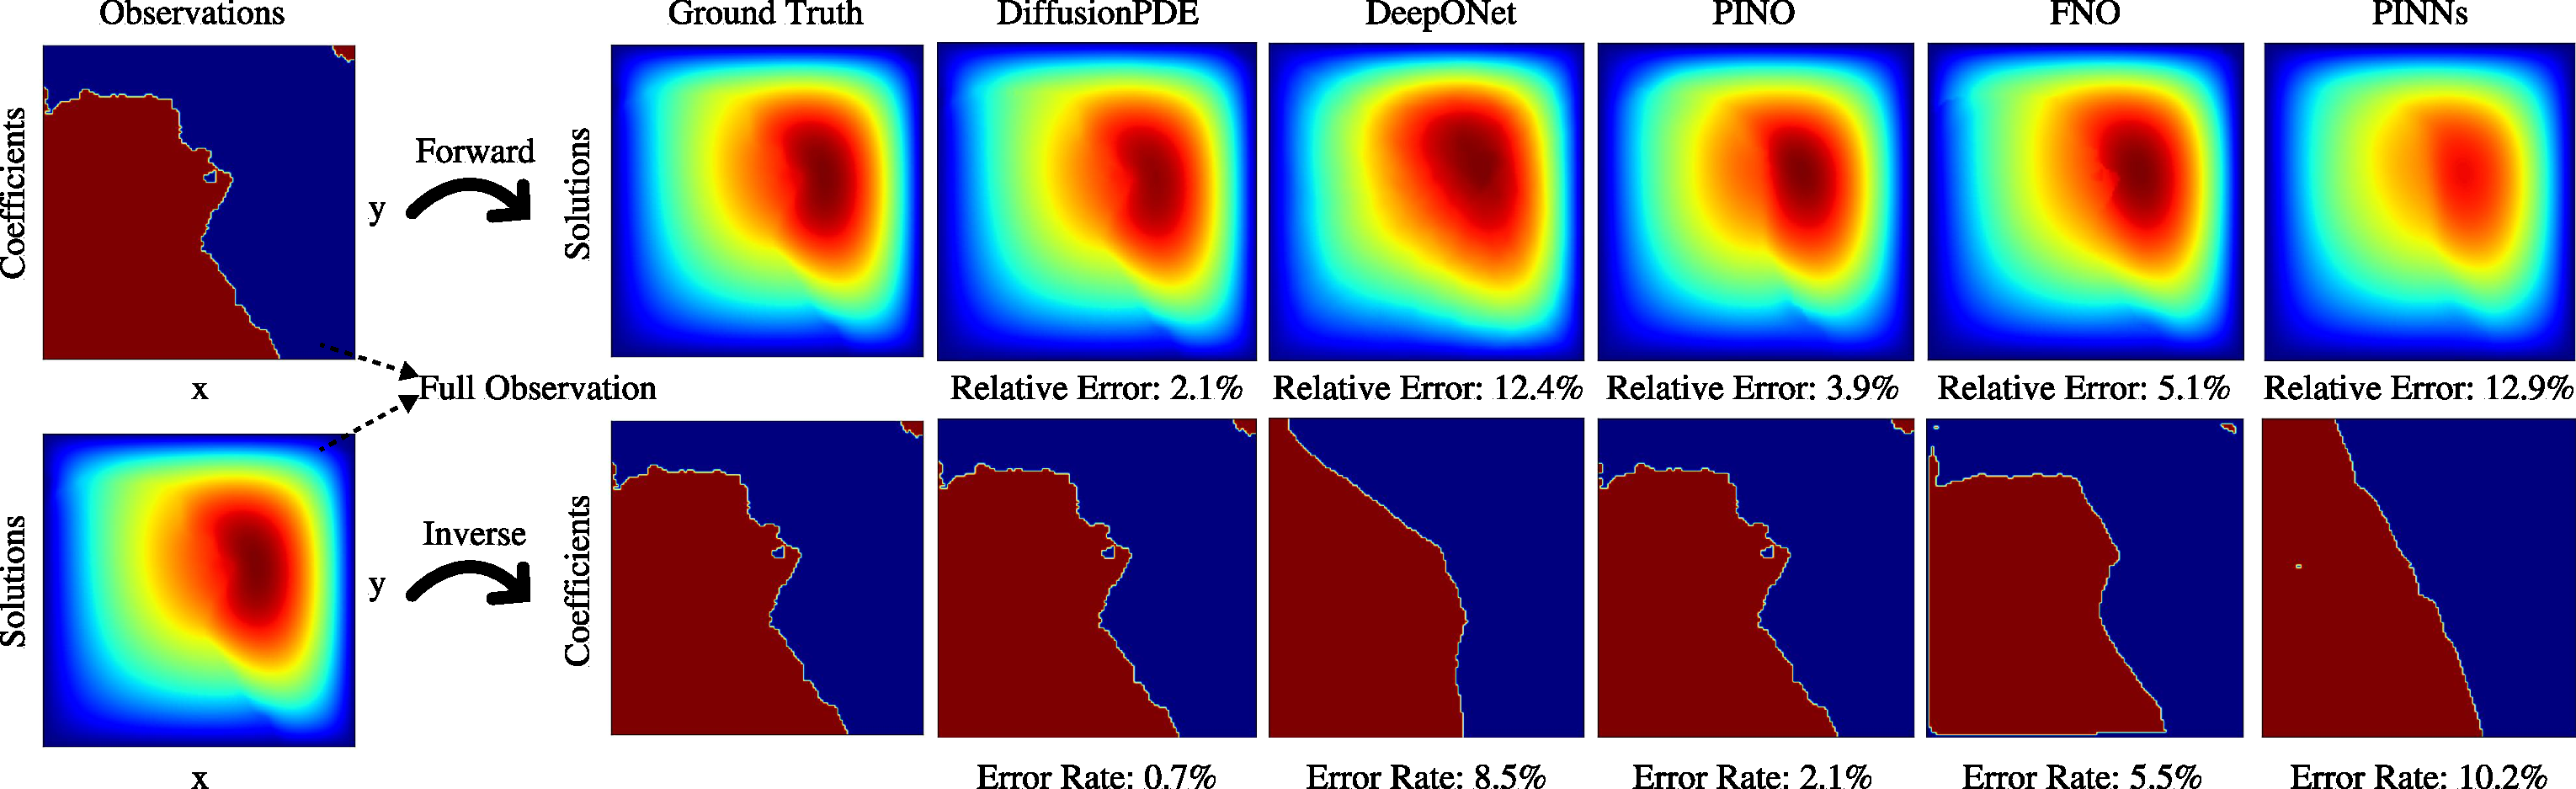
\includegraphics[width=0.99\textwidth]{figs/darcy/darcy_full_obs.pdf}
            \subcaption{Forward and inverse results of Darcy Flow recovered by full observation.}
            \vspace{0.3em}
        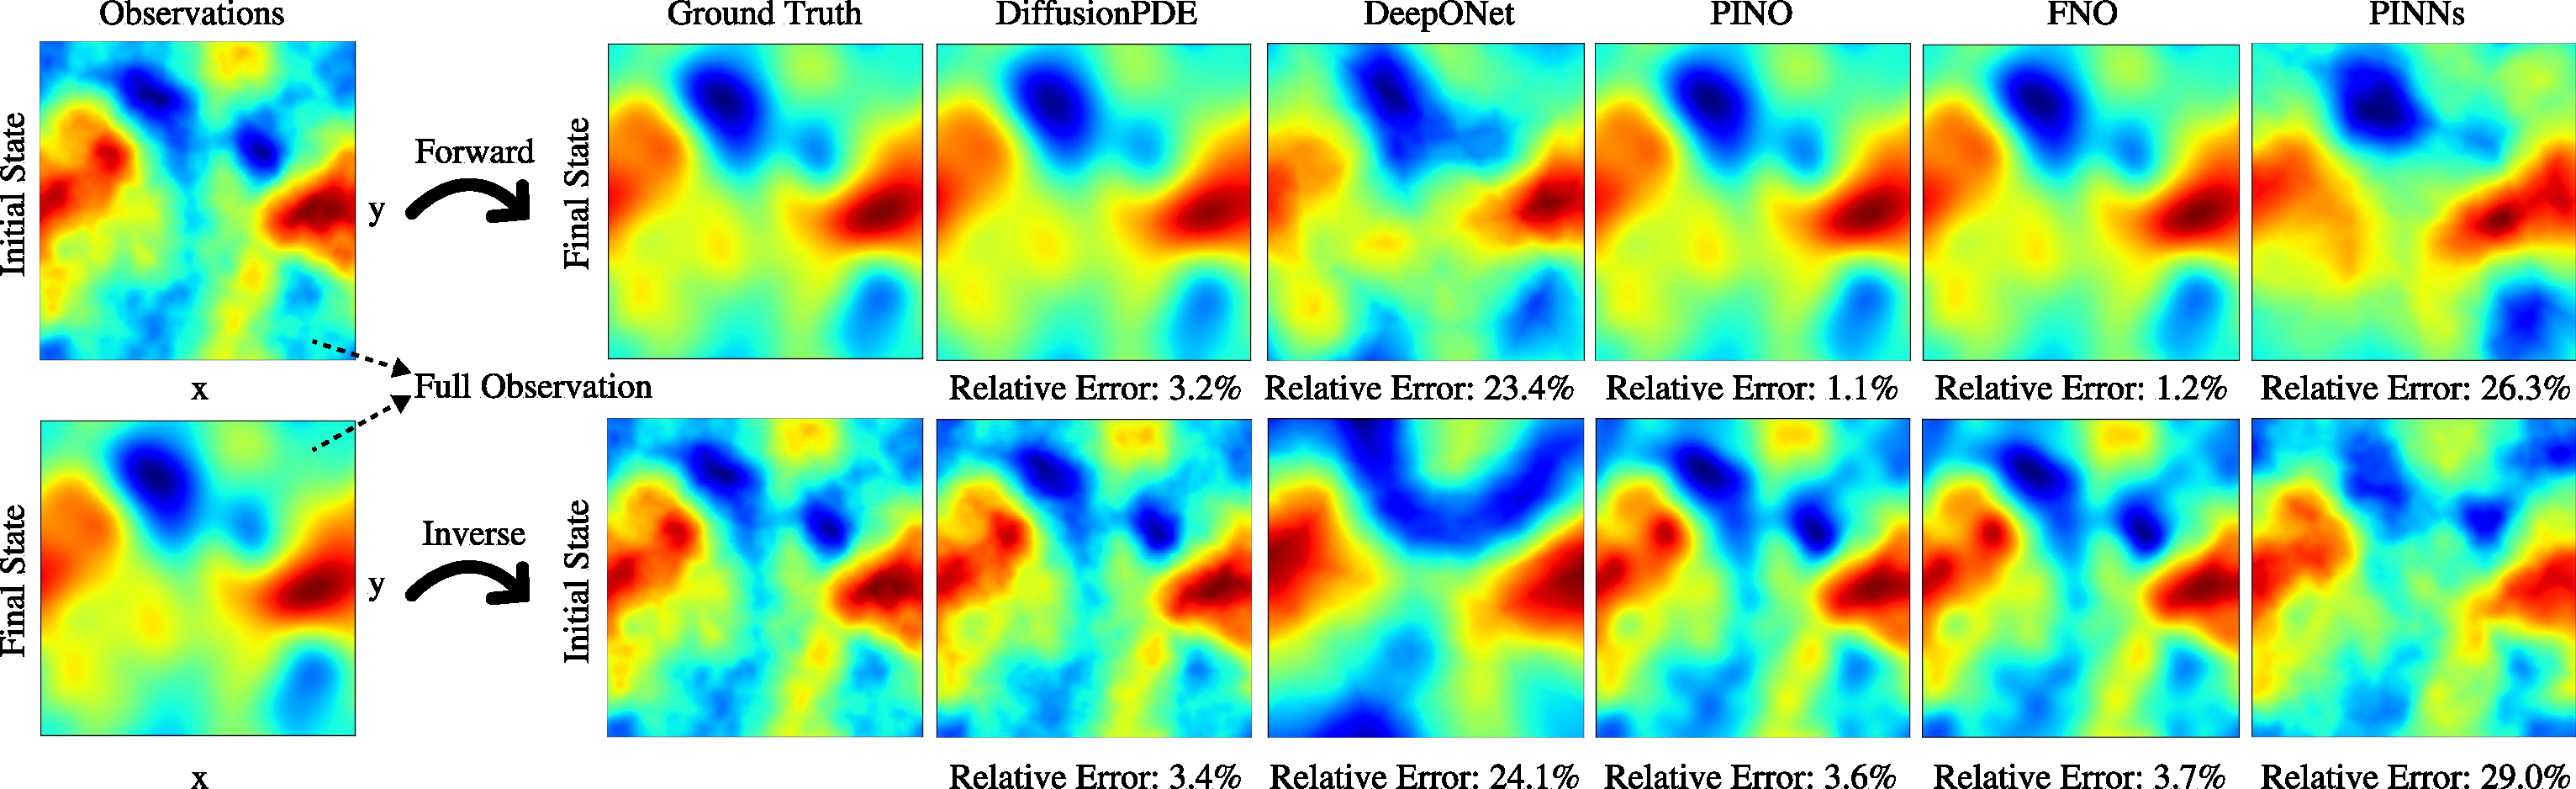
\includegraphics[width=0.99\textwidth]{figs/ns/ns_full_obs.pdf}
            \subcaption{Forward and inverse results of non-bounded Navier-Stokes equation recovered by full observation.}
        
    \end{subfigure}
    \caption{Results of forward and inverse problems for different PDE families with full observation.}
    \label{fig:pdes-full}
\end{figure}
\vspace{-1em}
\section{Training Baselines Methods on Partial Inputs}\label{sec:partialinput}
For our main experiments, we opt to train the baseline models (PINO, DeepONet, PINNs, FNO) on full observations for several compelling reasons: First, physics-informed models such as PINNs and PINO are unable to effectively compute the PDE loss when only sparse observations are available. Second, other models like DeepONet and FNO perform poorly with sparse observations. For instance, training the DeepONet model on 500 uniformly random points for each training sample in the context of the forward problem of Darcy Flow leads to testing outcomes that are consistently similar, as illustrated in Fig. \ref{fig:deeponet-partial}, regardless of the testing input. This pattern suggests that the model tends to generate a generalized solution that minimizes the average error across all potential solutions rather than converging based on specific samples. Furthermore, the partial-input-trained model exhibits poor generalization when faced with a different distribution of observations from training, indicating that it lacks flexibility—a critical attribute of our DiffusionPDE.

\begin{figure}[H]
    \centering
    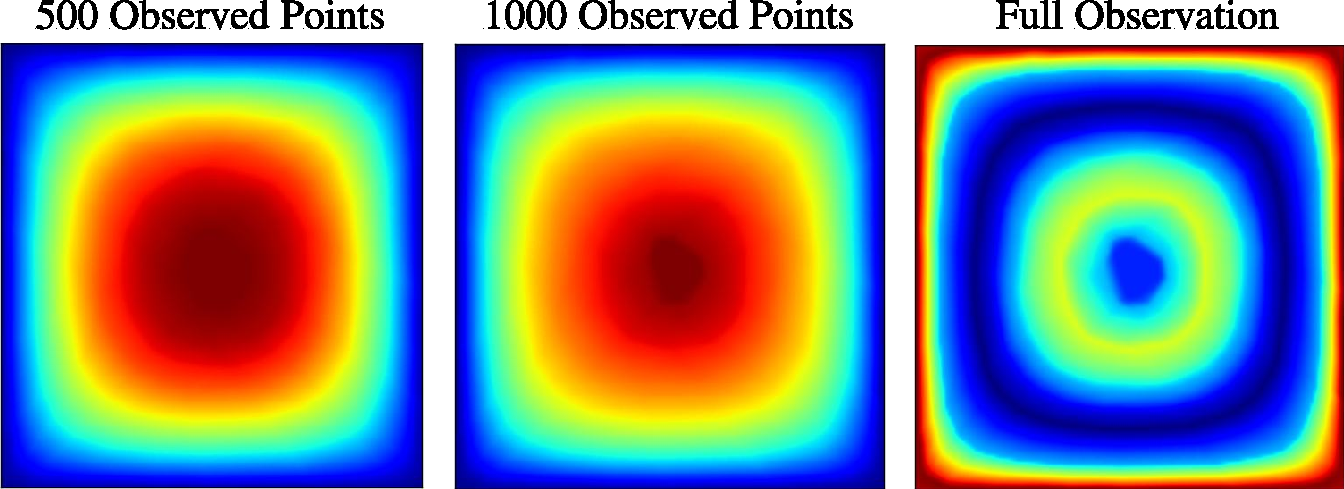
\includegraphics[width=0.6\textwidth]{figs/darcy/deeponet-partial-model.pdf}
    \caption{Predicted solutions obtained using the DeepONet model trained with 500 observation points across different numbers of observation points.}
    \label{fig:deeponet-partial}
\end{figure}
\vspace{-0.5em}


\section{Baseline Optimization}\label{sec:baseline-optimization}

We further refine the noisy outputs generated by baseline methods such as DeepONet, PINO, FNO, and PINNs. Specifically, given a partially observed parameter $\a$ for the PDE $f(\c; \a, \u) = 0$ and a pre-trained forward operator $\mathcal{F}'$, we address the problem by solving the optimization equation:
\begin{equation}
     \mathop{\min}_{a}\mathcal{L}_{pde}(\a, \mathcal{F}'(\a); f)
\end{equation}
and the results are shown in Table \ref{table:optimization-errors} and Fig. \ref{fig:optimization-poisson}. Optimization reduces errors and smooths the solutions. However, the resulting values are smaller due to the smoothing effect from minimizing PDE loss, and the overall error compared to the ground truth remains much higher than DiffusionPDE. This may be due to the difficulty in optimizing the derivatives of noisy $\a$ and $\u$.

\begin{table}[t!]
    \caption{Relative errors of solutions (or final states) and coefficients (or initial states) when solving forward and inverse problems respectively with sparse observations after optimizing the baselines. Error rates are used for the inverse problem of Darcy Flow.}
    \label{table:optimization-errors}
    \centering
    \begin{tabular}{p{3cm}lccccc}
        \toprule
        & & DiffusionPDE & DeepONet & PINO & FNO & PINNs \\
        \midrule
        \multirow{2}{*}{Darcy Flow} & Forward & \textbf{2.5\%} & 31.3\% & 32.6\% & 27.8\% & 6.9\% \\
        & Inverse & \textbf{3.2\%} & 41.1\% & 49.2\% & 49.3\% & 59.7\% \\
        \midrule
        \multirow{2}{*}{Poisson} & Forward & \textbf{4.5\%} & 73.6\% & 79.1\% & 70.5\% & 77.8\% \\
        & Inverse & \textbf{20.0\%} & 75.0\% & 115.0\% & 118.5\% & 73.9\% \\
        \midrule
        \multirow{2}{*}{Helmholtz} & Forward & \textbf{8.8\%} & 77.6\% & 67.7\% & 84.8\% & 79.2\% \\
        & Inverse & \textbf{22.6\%} & 100.7\% & 125.3\% & 131.6\% & 103.7\% \\
        \midrule
        \multirow{2}{3cm}{Non-bounded Navier-Stokes} & Forward & \textbf{6.9\%} & 96.5\% & 93.3\% & 91.6\% & 106.1\% \\
        & Inverse & \textbf{10.4\%} & 71.9\% & 87.8\% & 89.3\% & 108.6\% \\
        \midrule
        \multirow{2}{3cm}{Bounded Navier-Stokes} & Forward & \textbf{3.9\%} & 89.1\% & 80.8\% & 81.2\% & 84.4\% \\
        & Inverse & \textbf{2.7\%} & 88.6\% & 47.3\% & 48.7\% & 82.1\% \\
        \bottomrule
    \end{tabular}
\end{table}

\begin{figure}[t]
    \centering
    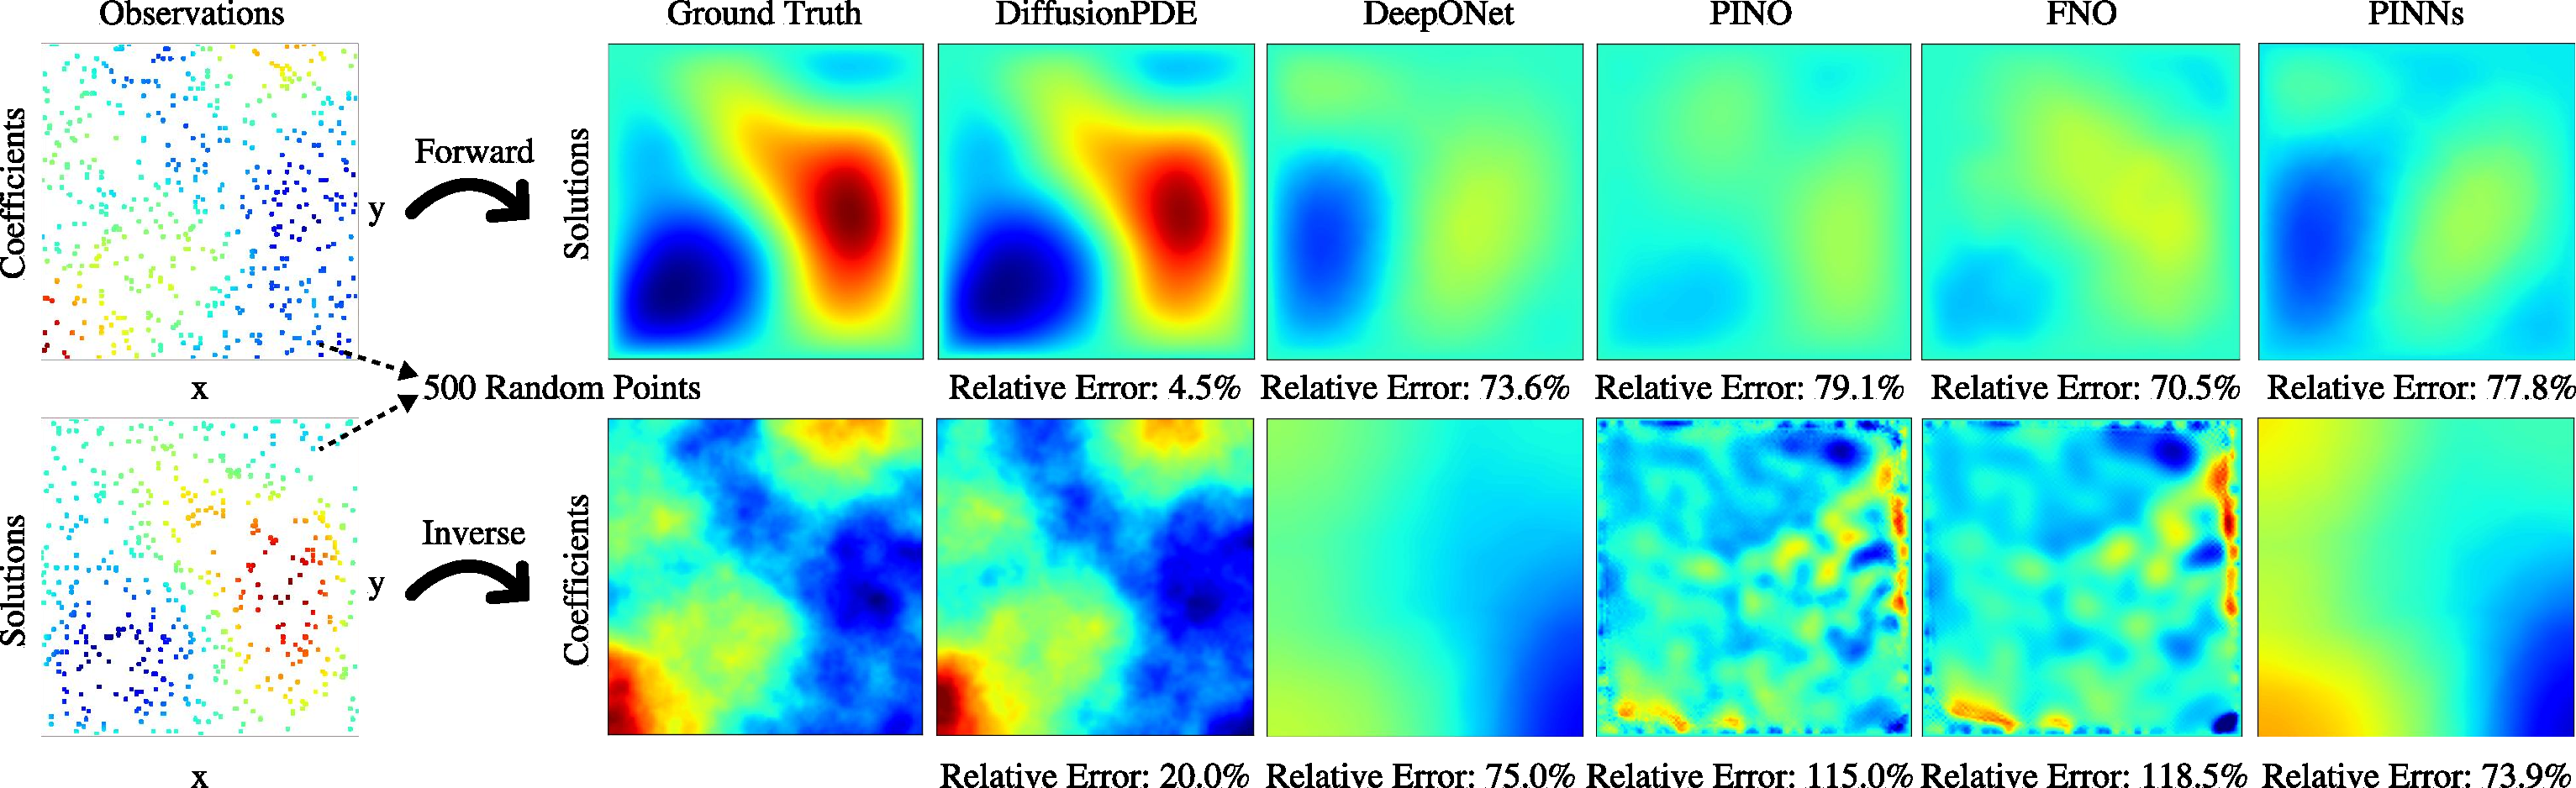
\includegraphics[width=0.99\textwidth]{figs/rebuttal/DiffusionPDE_31.pdf}
    \caption{Results of Poisson equation after optimizing baseline methods.}
    \label{fig:optimization-poisson}
\end{figure}


\section{Standard Deviation of DiffusionPDE Experiment Results}\label{sec:sd}

\vspace{-0.3em}

We further assess the statistical significance of our DiffusionPDE by analyzing the standard deviations for forward and inverse problems under conditions of 500 sparse observation points and full observation, respectively, as detailed in Table \ref{table:sd}. We evaluate our model using test sets comprising 1,000 samples for each PDE. Our findings confirm that full observation enhances the stability of the results, a predictable outcome as variability diminishes with an increase in observation points. The standard deviations are notably higher for more complex PDEs, such as the inverse problems of the Poisson and Helmholtz equations, reflecting the inherent challenges associated with these computations. Overall, DiffusionPDE demonstrates considerable stability, evidenced by relatively low standard deviations across various tests.

\vspace{-1em}

\begin{table}[H]
    \caption{Standard deviation of DiffusionPDE when solving forward and inverse problems with sparse or full observations.}
    \label{table:sd}
    \centering
    \begin{tabular}{p{2cm}lcc}
        \toprule
        & & Sparse Observations & Full Observations \\
        \midrule
        \multirow{2}{2cm}{Darcy Flow} & Forward & $2.5\pm 0.7\%$ & $2.2 \pm 0.1\%$ \\
        & Inverse & $3.2\pm 0.9\%$ & $2.0\pm 0.1\%$ \\
        \midrule
        \multirow{2}{2cm}{Poisson} & Forward & $4.5\pm 0.9\%$ & $2.7\pm 0.1\%$ \\
        & Inverse & $20.0\pm 1.8\%$ & $9.8\pm 0.7\%$ \\
        \midrule
        \multirow{2}{2cm}{Helmholtz} & Forward & $8.8\pm 1.0\%$ & $2.3\pm 0.1\%$ \\
        & Inverse & $22.6\pm 1.7\%$ & $4.0\pm 0.6\%$ \\
        \midrule
        \multirow{2}{2cm}{Non-bounded Navier-Stokes} & Forward & $6.9\pm 0.9\%$ & $6.1\pm 0.2\%$ \\
        & Inverse & $10.4\pm 1.0\%$ & $8.6\pm 0.3\%$ \\
        \midrule
        \multirow{2}{2cm}{Bounded Navier-Stokes} & Forward & $3.9\pm 0.2\%$ & $1.7\pm 0.1\%$ \\
        & Inverse & $2.7\pm 0.2\%$ & $1.4\pm 0.1\%$ \\
        \bottomrule
    \end{tabular}
\end{table}
\vspace{-0.5em}

\section{Runtime Analysis}\label{sec:runtime}
We evaluate the computing cost during the inference stage by testing a single data point on a single A40 GPU for the Navier-Stokes equation, as shown in Table \ref{table:cost}. DiffusionPDE has a lower computing cost compared to Shu et al. \cite{shu2023physics}, which autoregressively solves the full time interval. This advantage becomes more significant when we increase the number of time steps.

\begin{table}[H]
  \caption{Inference computing cost of sparse-observation-based methods.}
  \label{table:cost}
  \centering
  \begin{tabular}{lcccc}
    \toprule
    Method & DiffusionPDE (Ours) & GraphPDE & Shu et al. (2023) & OFormer \\
    \midrule
    \#Parameter (M) & 54 & 1.3 & 63 & 1.6 \\
    Inference time (s) & 140 & 84 & 180 & 3.2 \\
    GPU memory (GB) & 6.8 & 3.6 & 7.2 & 0.1 \\
    \bottomrule
  \end{tabular}
\end{table}

Further, we evaluate the inference runtimes on one single A40 GPU of vanilla full-observation-based methods and also the optimization time of them during the inference as introduced in Appendix \ref{sec:baseline-optimization}. The optimization runtimes are significantly slower, especially when using Fourier transforms.

\begin{table}[H]
  \caption{Average inference runtimes (in seconds) of full-observation-based methods with and without optimization.}
  \label{table:runtime-optimization}
  \centering
  \begin{tabular}{lcccc}
    \toprule
    Method & PINO & FNO & DeepONet & PINNs \\
    \midrule
    Vanilla & 1.0e0 & 9.8e-1 & 7.4e-1 & 1.5e0 \\
    With Optimization & 6.7e2 & 6.7e2 & 3.5e1 & 3.7e1 \\
    \bottomrule
  \end{tabular}
\end{table}

\vspace{-1em}
\section{Robustness of DiffusionPDE}\label{sec:robust}
\vspace{-0.5em}

We find that DiffusionPDE is robust against sparse noisy observation. In Fig. \ref{fig:robustness}, we add Gaussian noise to the 500 observed points of Darcy Flow coefficients. Our DiffusionPDE can maintain a relative error of around 10\% with a 15\% noise level concerning the forward problem, and the recovered solutions are shown in Fig. \ref{fig:darcy-robust-vis}. Baseline methods such as PINO also exhibit robustness against random noise under sparse observation conditions; this is attributed to their limited applicability to sparse observation problems, leading them to address the problem in a more randomized manner.

\vspace{-0.5em}
\begin{figure}[H]
    \centering
    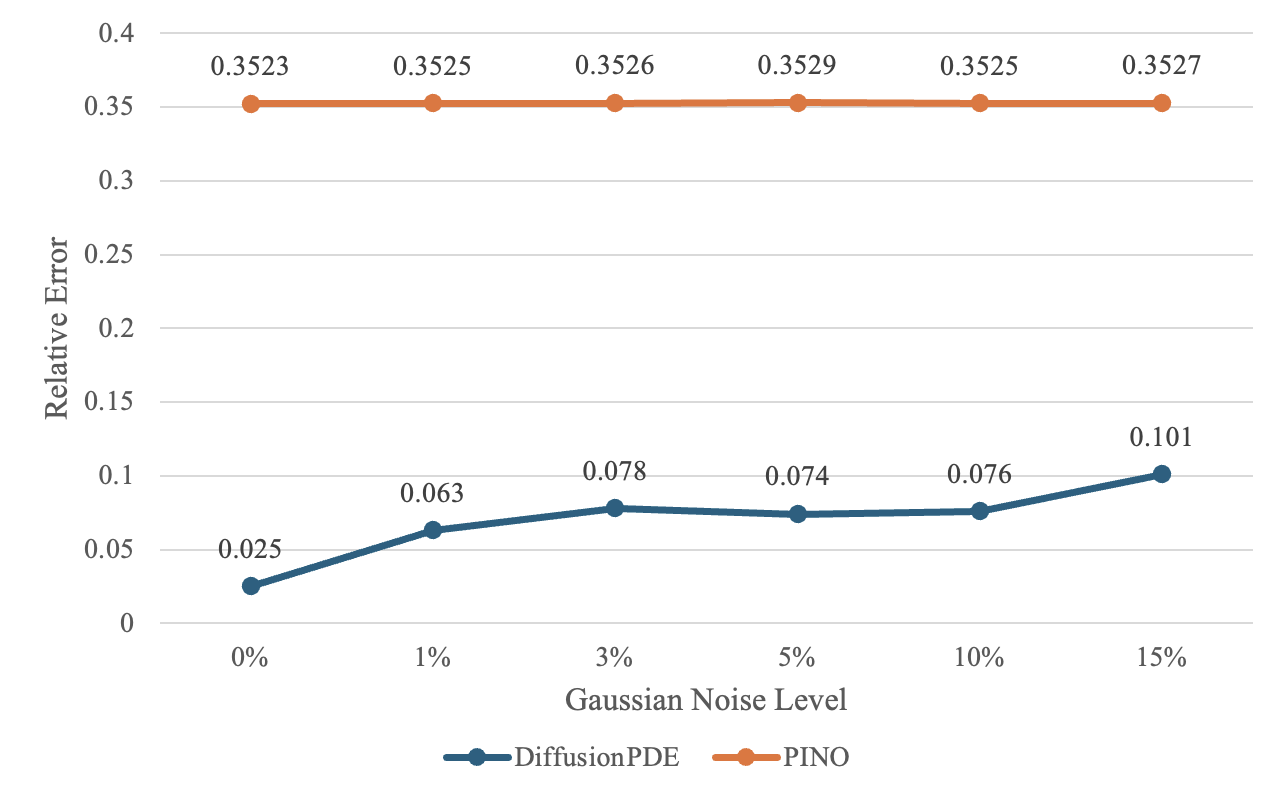
\includegraphics[width=0.7\textwidth]{figs/darcy/robustness.png}
    \vspace{-0.3em}
    \caption{Relative errors of recovered Darcy Flow solutions with sparse noisy observation.}
    \label{fig:robustness}
    \vspace{-1.0em}
\end{figure}

\begin{figure}[H]
    \centering
    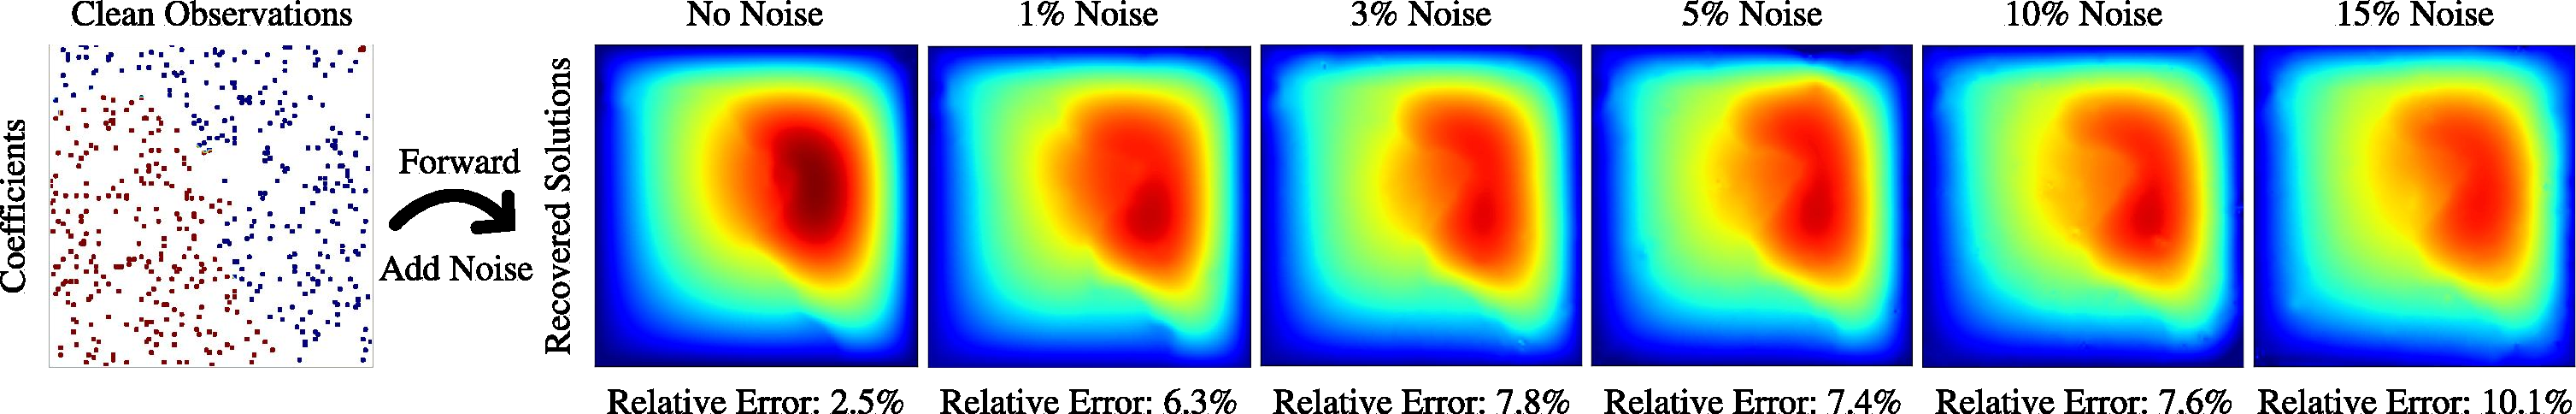
\includegraphics[width=0.99\textwidth]{figs/darcy/darcy_robustness_visualize.pdf}
    \vspace{-0.3em}
    \caption{Recovered solutions for Darcy Flow with noisy observations.}
    \label{fig:darcy-robust-vis}
\end{figure}

\vspace{-1.5em}
\paragraph{Robustness on Sampling Patterns} Moreover, as mentioned in the main document, we investigate the robustness of DiffusionPDE on different sampling patterns of the observation points.
Here, we address the forward problem of Darcy Flow using 500 observed coefficient points, which are non-uniformly concentrated on the left and right sides or are regularly distributed across the grid, as depicted in Fig. \ref{fig:darcy-different-obs}. Our results demonstrate that DiffusionPDE flexibly solves problems with arbitrary sparse observation locations within the spatial domain, without re-training the neural network model. However, the CFG method faces challenges when solving with varying sampling patterns, as demonstrated in Fig. \ref{fig:diff-patter-cfg}. In this figure, we compare the reconstruction results of DiffusionPDE and Diffusion with CFG for the unbounded Navier-Stokes equation, where all observation points are located on the left side of the grid. The CFG approach struggles with this asymmetric sampling pattern, while DiffusionPDE maintains more accurate reconstructions.

\vspace{-0.5em}
\begin{figure}[H]
    \centering
    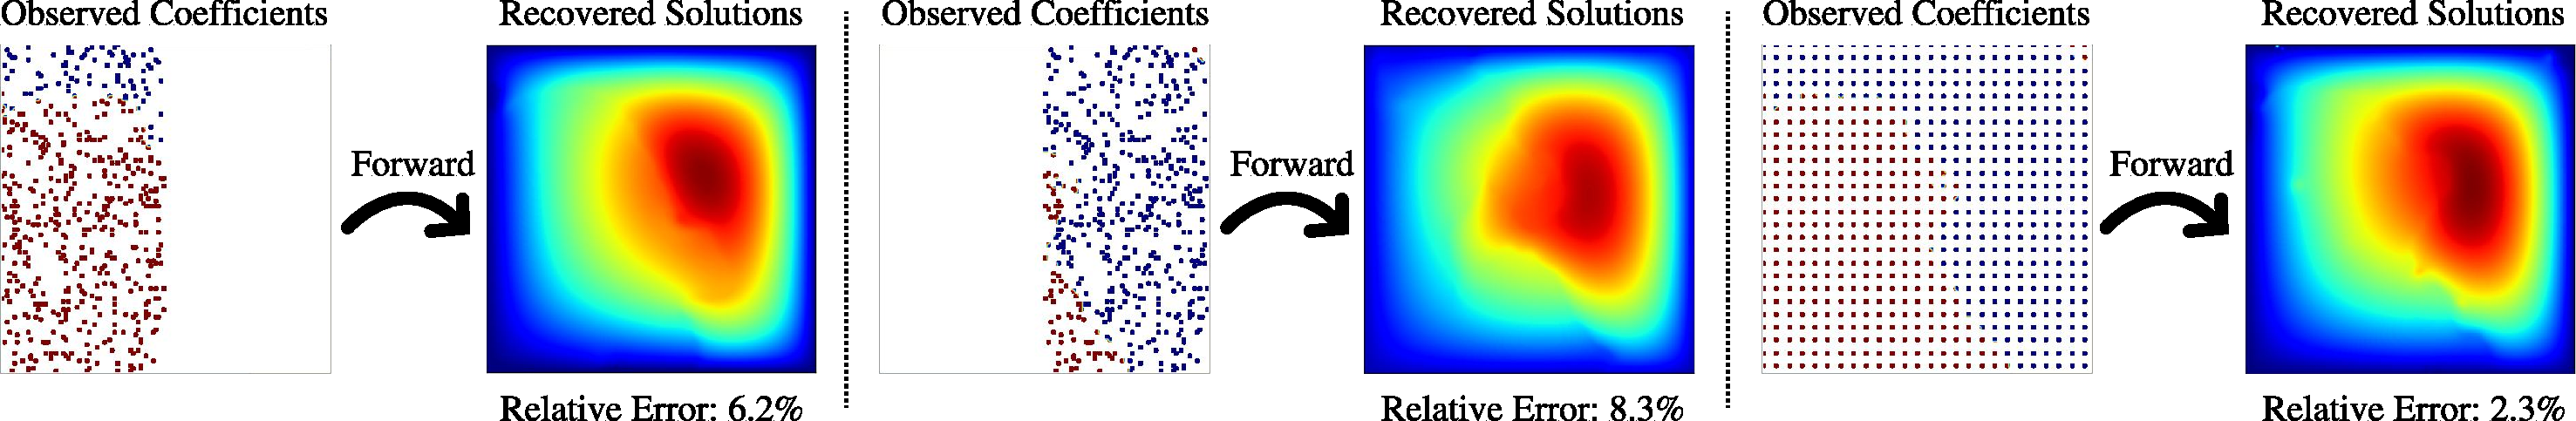
\includegraphics[width=0.99\textwidth]{figs/darcy/darcy_obs_different.pdf}
    \vspace{-0.2em}
    \caption{Recovered solutions for Darcy Flow with observations sampled using non-uniform distributions.}
    \label{fig:darcy-different-obs}
    \vspace{-0.5em}
\end{figure}

\begin{figure}[H]
    \centering
    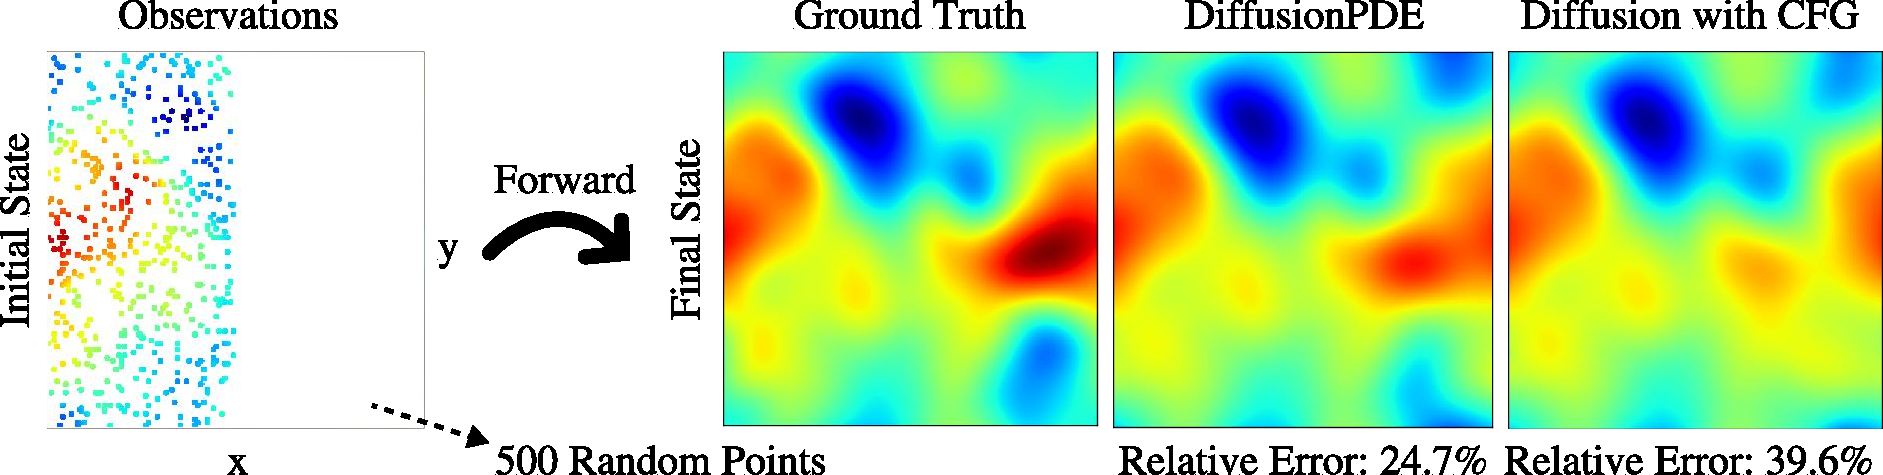
\includegraphics[width=0.7\textwidth]{figs/rebuttal/DiffusionPDE_37.pdf}
    \caption{Comparison between DiffusionPDE and Diffusion CFG under different sampling patterns for non-bounded Navier-Stokes equation.}
    \label{fig:diff-patter-cfg}
\end{figure}

\vspace{-1.0em}

\paragraph{Stochasticity Evaluation}

Since we employ a deterministic diffusion model, with partial observations as input, the only source of stochasticity or uncertainty in our approach arises from the initial random noise. To examine this, we conducted experiments to assess the impact of different noise seeds on both the initial and final states of the Navier-Stokes equations, as demonstrated in Fig. \ref{fig:diff-initial-noise}. Our findings indicate that the diffusion model exhibits some degree of uncertainty in its predictions, despite the deterministic nature of the underlying framework.
\vspace{-0.5em}
\begin{figure}[H]
    \centering
    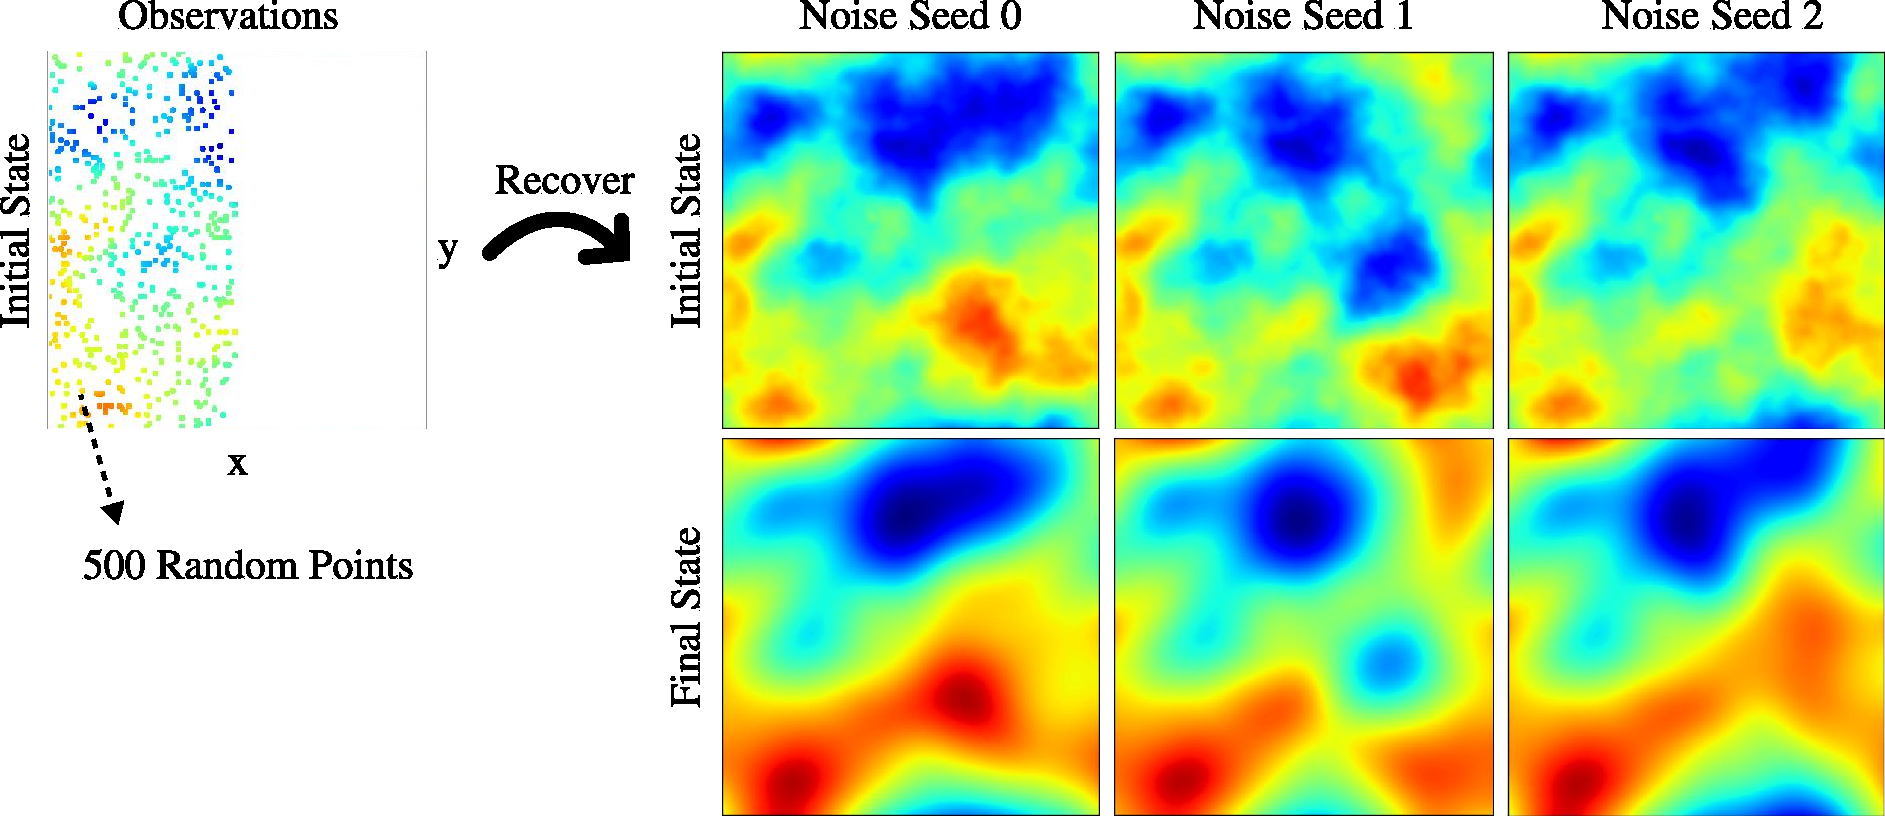
\includegraphics[width=0.7\textwidth]{figs/rebuttal/DiffusionPDE_26.pdf}
    \vspace{-0.2em}
    \caption{Different predictions of DiffusionPDE generated by different initial noise for non-bounded Navier-Stokes equation.}
    \label{fig:diff-initial-noise}
    \vspace{-1em}
\end{figure}


\section{Solving Forward and Inverse Problems with Different Numbers of Observations}\label{sec:different_num_obs}

We also investigate how our DiffusionPDE handles varying degrees of sparse observation. Experiments are conducted on the Darcy Flow, Poisson equation, Helmholtz equation, and non-bounded Navier-Stokes equation. We examine the results of DiffusionPDE in solving forward and inverse problems when there are $100$, $300$, $500$, and $1000$ random observations on $a$, $u$, or both $a$ and $u$, as shown in Fig. \ref{fig:abalation-different-observation-num}. We have observed that the error of DiffusionPDE decreases as the number of sparse observations increases. Overall, we recover $u$ better than $a$. DiffusionPDE can recover $u$ with approximately $2\%$ observation points at any side pretty well. DiffusionPDE is also capable of recovering both $a$ and $u$ with errors $1\%\sim10\%$ with approximately $6\%$ observation points at any side for most PDE families. We also conclude that our DiffusionPDE becomes insensitive to the number of observations once more than $3\%$ of the points are observed.

\begin{figure}[H]
    
        \begin{subfigure}{\textwidth}
        \centering
        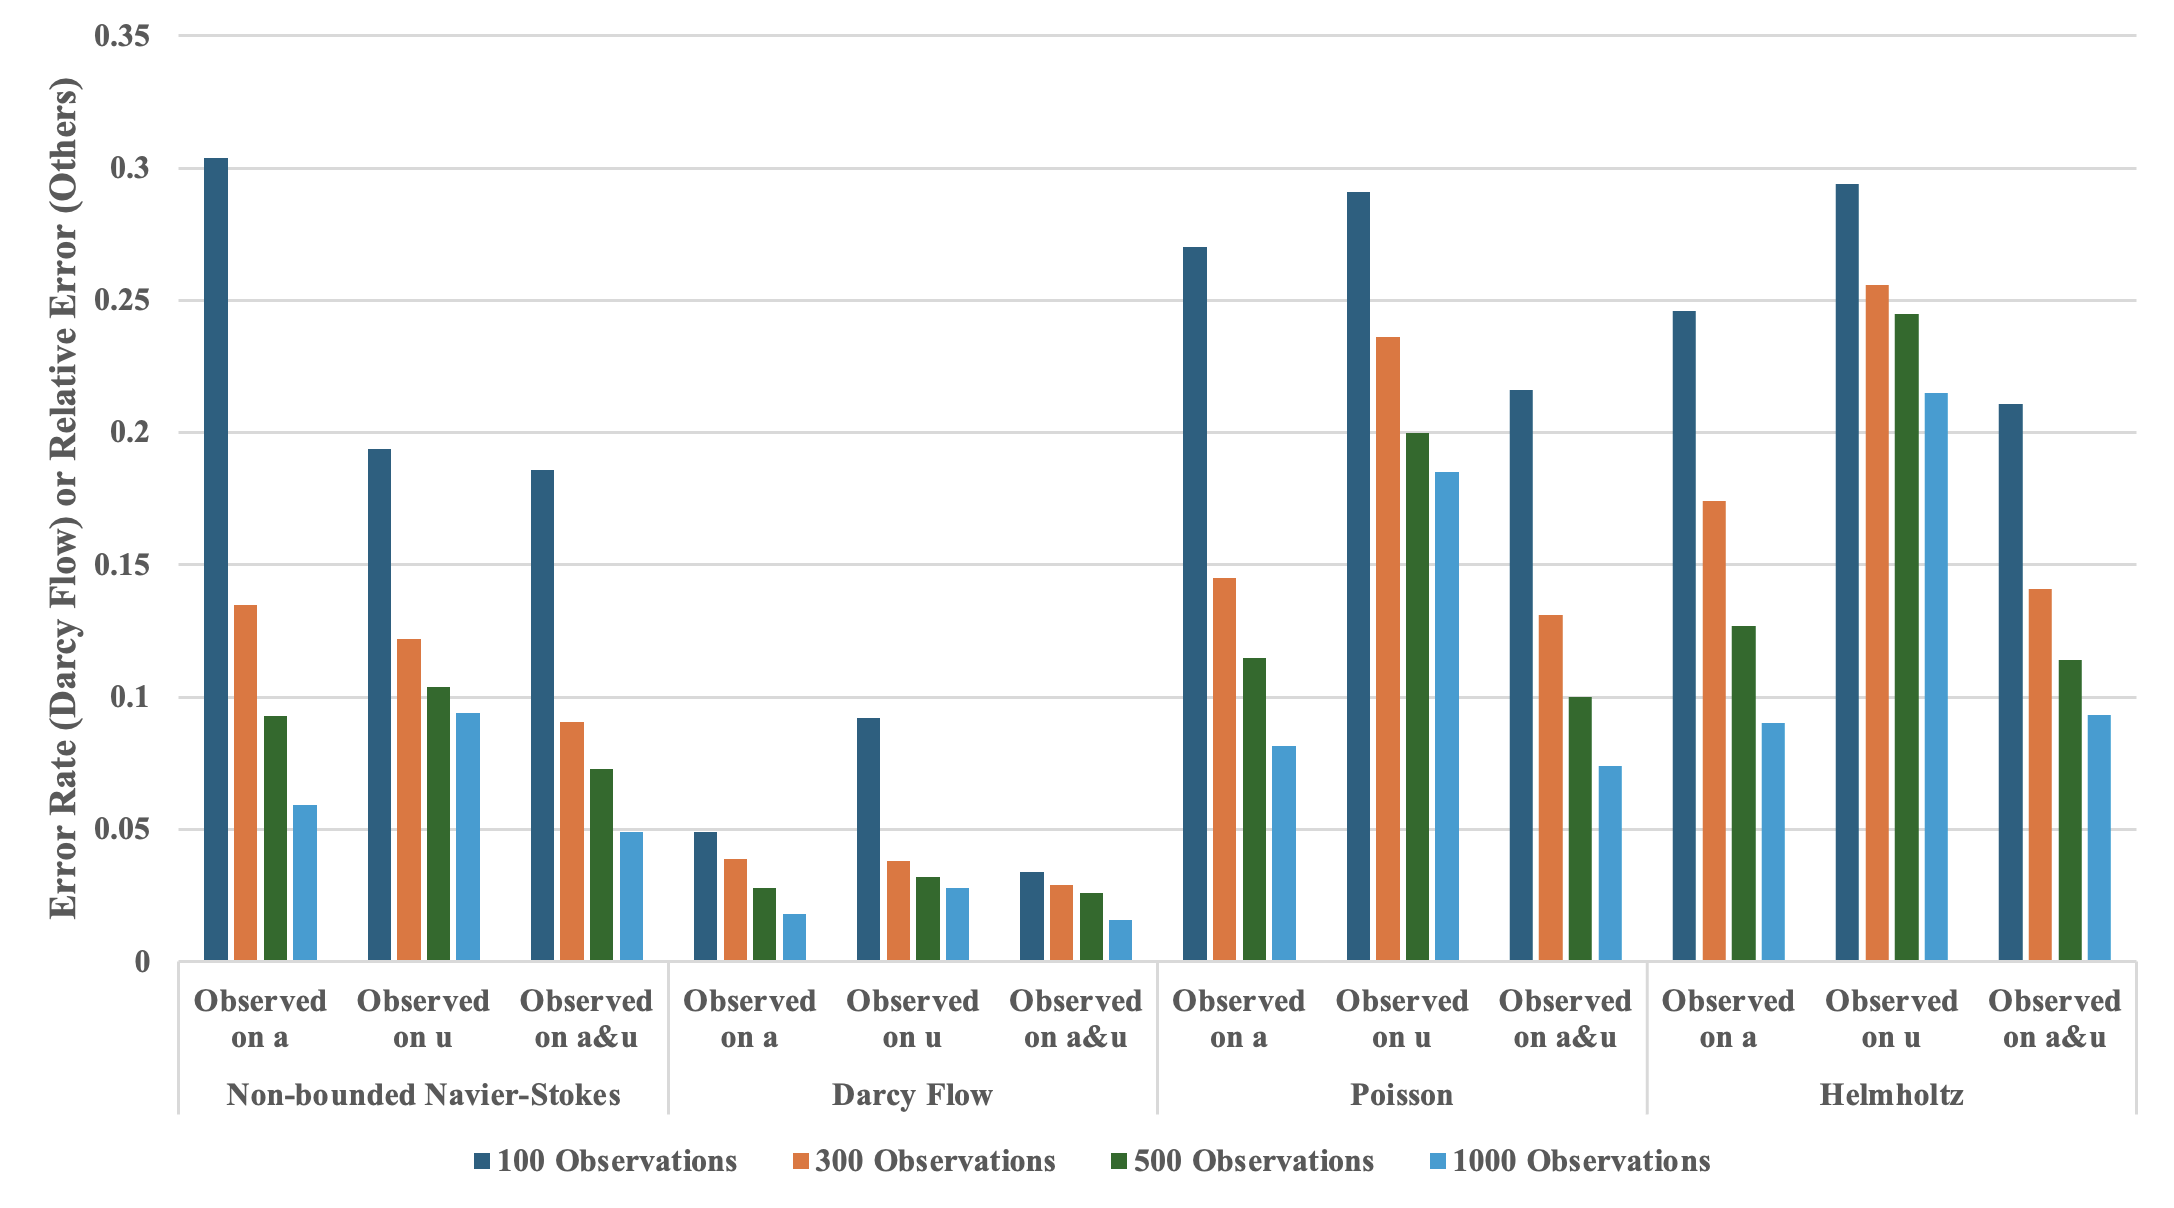
\includegraphics[width=0.99\textwidth]{figs/ablation/differentobsnum_inverse.png}
            \subcaption{Error rates for Darcy Flow and relative errors for other PDEs of recovered coefficients or initial states $a$.}
        \end{subfigure}
\end{figure}
\begin{figure}[H] \ContinuedFloat
        \begin{subfigure}{\textwidth}
        \centering
            % \vspace{0.8em}
            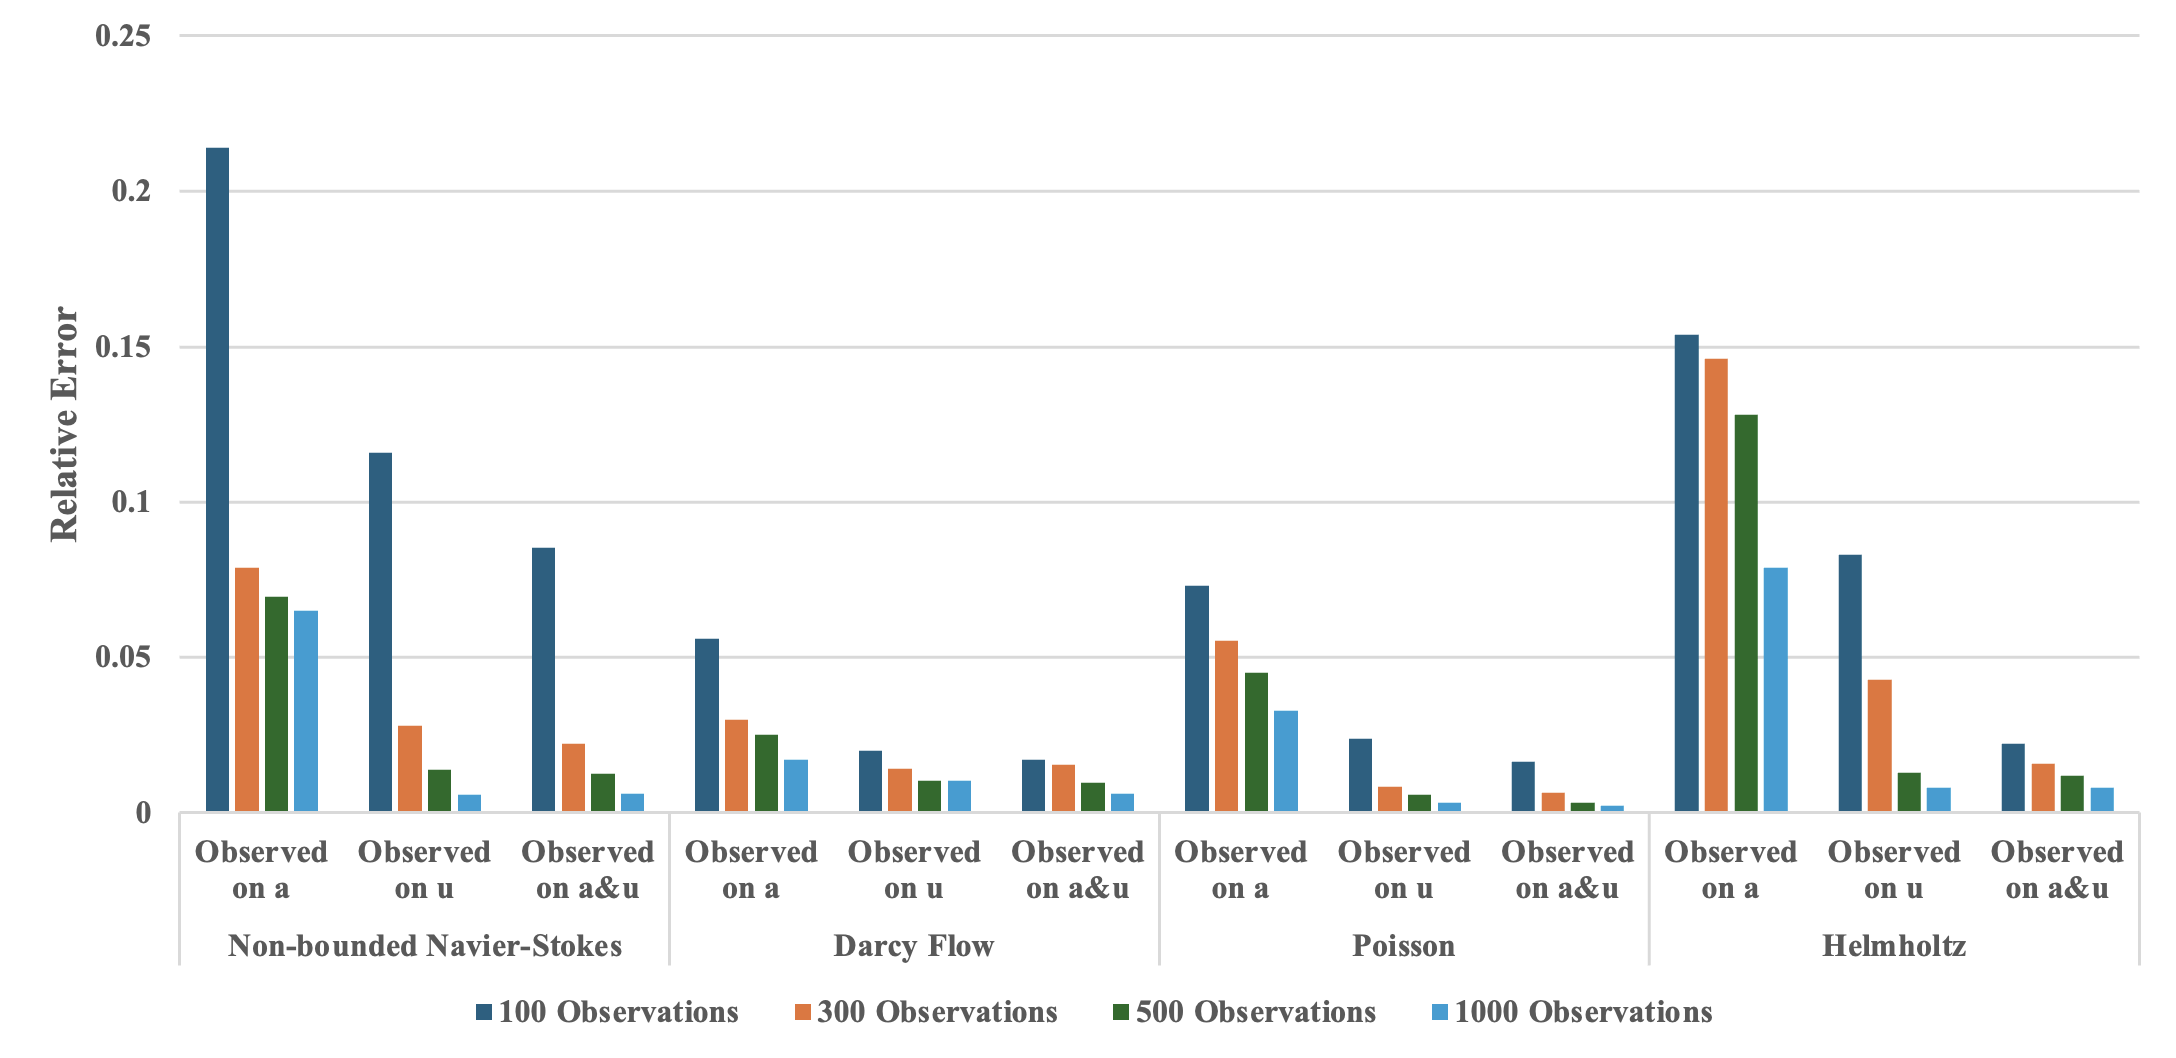
\includegraphics[width=0.99\textwidth]{figs/ablation/differentobsnum_forward.png}  
            \subcaption{Relative errors of recovered solutions or final states $u$.}
        \end{subfigure}
    \caption{Error rate or relative error of both coefficients (or initial states) $a$ and solutions (or final states) $u$ with different numbers of observations.}
    \label{fig:abalation-different-observation-num}
\end{figure}

\section{Solving Forward and Inverse Problems across Varied Resolutions} \label{sec:different-resolution}

To evaluate the generalizability of DiffusionPDE, we implemented the model on various resolutions, including $64\times 64$ and $256\times 256$, while maintaining the same percentage of observed points. For resolutions of $64\times 64$, $128\times 128$, and $256\times 256$, we observe $125$, $500$, and $2000$ points on $a$ or $u$ respectively, which are approximately $3\%$ for each resolution. Overall, DiffusionPDE is capable of handling different resolutions effectively. For instance, Table \ref{table:different-resolution} presents the forward relative errors of the solution $u$ and inverse error rates of the coefficient $a$ for the Darcy Flow, demonstrating that DiffusionPDE performs consistently well with similar error rates across various resolutions.

\begin{table}[H]
  \caption{Forward relative errors and inverse error rates of Darcy Flow across different resolutions.}
  \label{table:different-resolution}
  \centering
  \begin{tabular}{ccc}
    \toprule
    Resolution & Forward Relative Error & Inverse Error Rate \\
    \midrule
    $64\times 64$ & $2.9\%$ & $4.3\%$ \\
    $128\times 128$ & $2.5\%$ & $3.2\%$ \\
    $256\times 256$ & $3.1\%$ & $4.1\%$ \\
    \bottomrule
  \end{tabular}
\end{table}

\section{Comparison with Other Baselines}\label{sec:other-baseline}

We have compared the results using the RBF kernel \cite{bollig2012solution}, as shown in Fig. \ref{fig:rbf}. For the forward process of solving the Poisson, Helmholtz, and Darcy Flow equations, the RBF kernel achieved solution errors of approximately $14.3\%$, $23.1\%$, and $18.4\%$, respectively, with 500 random observation points. However, when addressing the inverse problem, the errors increased significantly to $141.2\%$, $143.1\%$, and $34.0\%$, respectively. This increase in error is likely due to the inherent challenges of solving inverse problems with such a straightforward method.

\begin{figure}[H]
    \centering
    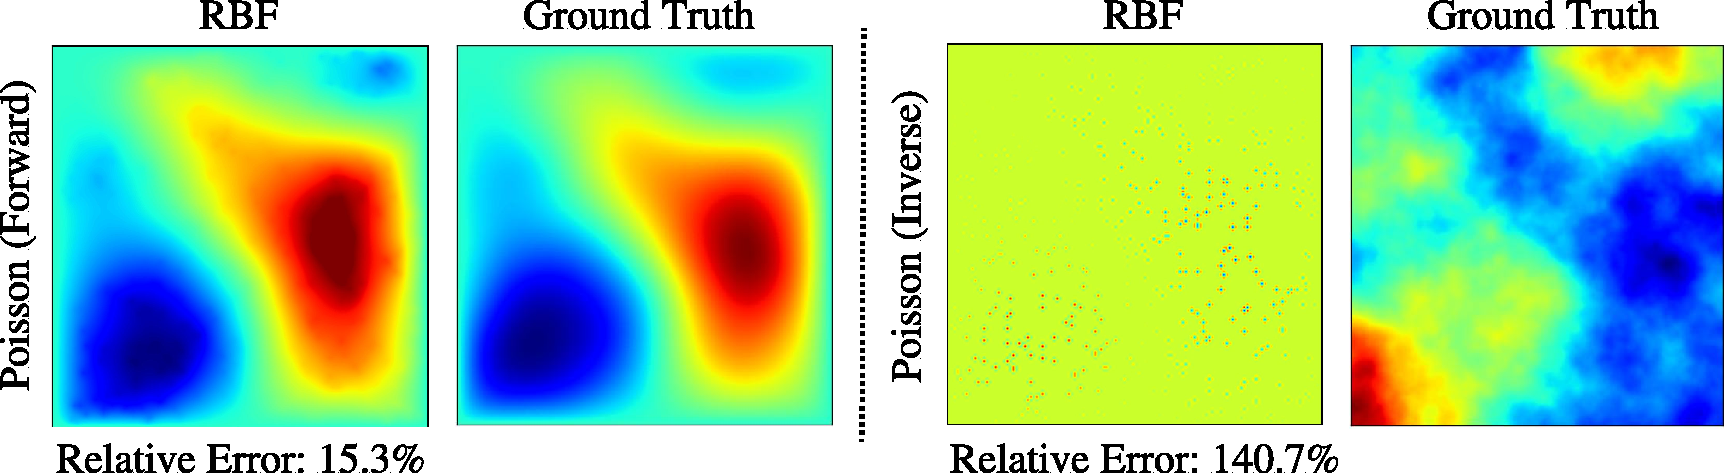
\includegraphics[width=0.7\textwidth]{figs/rebuttal/DiffusionPDE_27.pdf}
    \caption{Forward and Inverse Results of Poisson equation recovered by 500 observation points using RBF Kernel.}
    \label{fig:rbf}
\end{figure}

Additionally, we compare our DiffusionPDE method with a single U-Net model. The U-Net is trained based on our EDM diffusion model, where we initially train it to map between 500 fixed input points and the full output space, as illustrated in Fig. \ref{fig:unet}. For the Navier-Stokes equation, the prediction of the final state results in an average test error of approximately 39\%, which is significantly higher than the error produced by our diffusion model. Furthermore, when making predictions using 500 different sampling points, the relative error increases to approximately 49\%. We also train another U-Net model to map between 500 random input points and the full output space, but this model results in a test error of 101\%, indicating that the U-Net struggles to adapt to varying sampling patterns and fails to flexibly solve different configurations.

\begin{figure}[H]
    \centering
    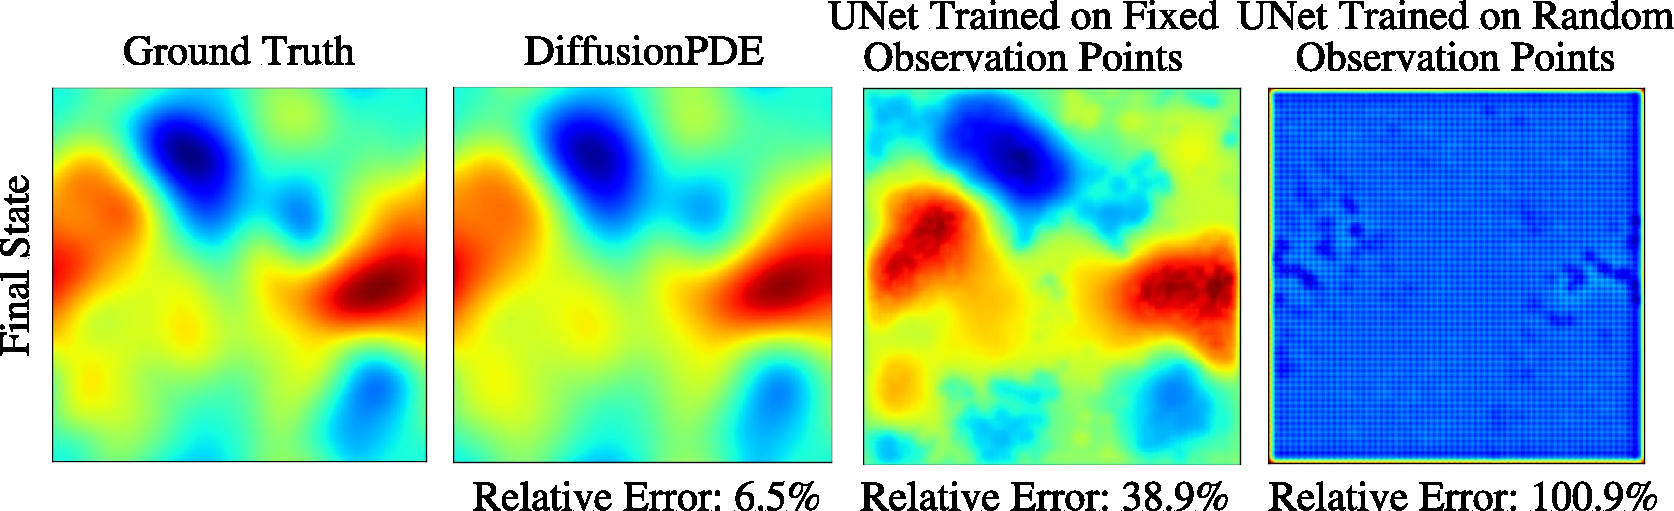
\includegraphics[width=0.7\textwidth]{figs/rebuttal/DiffusionPDE_34.pdf}
    \caption{Comparison between DiffusionPDE and U-Net regarding non-bounded Navier-Stokes equation.}
    \label{fig:unet}
\end{figure}


